% Options for packages loaded elsewhere
\PassOptionsToPackage{unicode}{hyperref}
\PassOptionsToPackage{hyphens}{url}
\PassOptionsToPackage{dvipsnames,svgnames,x11names}{xcolor}
%
\documentclass[
  bookmarksnumbered]{article}
\usepackage{amsmath,amssymb}
\usepackage{iftex}
\ifPDFTeX
  \usepackage[T1]{fontenc}
  \usepackage[utf8]{inputenc}
  \usepackage{textcomp} % provide euro and other symbols
\else % if luatex or xetex
  \usepackage{unicode-math} % this also loads fontspec
  \defaultfontfeatures{Scale=MatchLowercase}
  \defaultfontfeatures[\rmfamily]{Ligatures=TeX,Scale=1}
\fi
\usepackage{lmodern}
\ifPDFTeX\else
  % xetex/luatex font selection
\fi
% Use upquote if available, for straight quotes in verbatim environments
\IfFileExists{upquote.sty}{\usepackage{upquote}}{}
\IfFileExists{microtype.sty}{% use microtype if available
  \usepackage[]{microtype}
  \UseMicrotypeSet[protrusion]{basicmath} % disable protrusion for tt fonts
}{}
\makeatletter
\@ifundefined{KOMAClassName}{% if non-KOMA class
  \IfFileExists{parskip.sty}{%
    \usepackage{parskip}
  }{% else
    \setlength{\parindent}{0pt}
    \setlength{\parskip}{6pt plus 2pt minus 1pt}}
}{% if KOMA class
  \KOMAoptions{parskip=half}}
\makeatother
\usepackage{xcolor}
\usepackage[margin=2cm]{geometry}
\usepackage{color}
\usepackage{fancyvrb}
\newcommand{\VerbBar}{|}
\newcommand{\VERB}{\Verb[commandchars=\\\{\}]}
\DefineVerbatimEnvironment{Highlighting}{Verbatim}{commandchars=\\\{\}}
% Add ',fontsize=\small' for more characters per line
\usepackage{framed}
\definecolor{shadecolor}{RGB}{48,48,48}
\newenvironment{Shaded}{\begin{snugshade}}{\end{snugshade}}
\newcommand{\AlertTok}[1]{\textcolor[rgb]{1.00,0.81,0.69}{#1}}
\newcommand{\AnnotationTok}[1]{\textcolor[rgb]{0.50,0.62,0.50}{\textbf{#1}}}
\newcommand{\AttributeTok}[1]{\textcolor[rgb]{0.80,0.80,0.80}{#1}}
\newcommand{\BaseNTok}[1]{\textcolor[rgb]{0.86,0.64,0.64}{#1}}
\newcommand{\BuiltInTok}[1]{\textcolor[rgb]{0.80,0.80,0.80}{#1}}
\newcommand{\CharTok}[1]{\textcolor[rgb]{0.86,0.64,0.64}{#1}}
\newcommand{\CommentTok}[1]{\textcolor[rgb]{0.50,0.62,0.50}{#1}}
\newcommand{\CommentVarTok}[1]{\textcolor[rgb]{0.50,0.62,0.50}{\textbf{#1}}}
\newcommand{\ConstantTok}[1]{\textcolor[rgb]{0.86,0.64,0.64}{\textbf{#1}}}
\newcommand{\ControlFlowTok}[1]{\textcolor[rgb]{0.94,0.87,0.69}{#1}}
\newcommand{\DataTypeTok}[1]{\textcolor[rgb]{0.87,0.87,0.75}{#1}}
\newcommand{\DecValTok}[1]{\textcolor[rgb]{0.86,0.86,0.80}{#1}}
\newcommand{\DocumentationTok}[1]{\textcolor[rgb]{0.50,0.62,0.50}{#1}}
\newcommand{\ErrorTok}[1]{\textcolor[rgb]{0.76,0.75,0.62}{#1}}
\newcommand{\ExtensionTok}[1]{\textcolor[rgb]{0.80,0.80,0.80}{#1}}
\newcommand{\FloatTok}[1]{\textcolor[rgb]{0.75,0.75,0.82}{#1}}
\newcommand{\FunctionTok}[1]{\textcolor[rgb]{0.94,0.94,0.56}{#1}}
\newcommand{\ImportTok}[1]{\textcolor[rgb]{0.80,0.80,0.80}{#1}}
\newcommand{\InformationTok}[1]{\textcolor[rgb]{0.50,0.62,0.50}{\textbf{#1}}}
\newcommand{\KeywordTok}[1]{\textcolor[rgb]{0.94,0.87,0.69}{#1}}
\newcommand{\NormalTok}[1]{\textcolor[rgb]{0.80,0.80,0.80}{#1}}
\newcommand{\OperatorTok}[1]{\textcolor[rgb]{0.94,0.94,0.82}{#1}}
\newcommand{\OtherTok}[1]{\textcolor[rgb]{0.94,0.94,0.56}{#1}}
\newcommand{\PreprocessorTok}[1]{\textcolor[rgb]{1.00,0.81,0.69}{\textbf{#1}}}
\newcommand{\RegionMarkerTok}[1]{\textcolor[rgb]{0.80,0.80,0.80}{#1}}
\newcommand{\SpecialCharTok}[1]{\textcolor[rgb]{0.86,0.64,0.64}{#1}}
\newcommand{\SpecialStringTok}[1]{\textcolor[rgb]{0.80,0.58,0.58}{#1}}
\newcommand{\StringTok}[1]{\textcolor[rgb]{0.80,0.58,0.58}{#1}}
\newcommand{\VariableTok}[1]{\textcolor[rgb]{0.80,0.80,0.80}{#1}}
\newcommand{\VerbatimStringTok}[1]{\textcolor[rgb]{0.80,0.58,0.58}{#1}}
\newcommand{\WarningTok}[1]{\textcolor[rgb]{0.50,0.62,0.50}{\textbf{#1}}}
\usepackage{longtable,booktabs,array}
\usepackage{calc} % for calculating minipage widths
% Correct order of tables after \paragraph or \subparagraph
\usepackage{etoolbox}
\makeatletter
\patchcmd\longtable{\par}{\if@noskipsec\mbox{}\fi\par}{}{}
\makeatother
% Allow footnotes in longtable head/foot
\IfFileExists{footnotehyper.sty}{\usepackage{footnotehyper}}{\usepackage{footnote}}
\makesavenoteenv{longtable}
\usepackage{graphicx}
\makeatletter
\def\maxwidth{\ifdim\Gin@nat@width>\linewidth\linewidth\else\Gin@nat@width\fi}
\def\maxheight{\ifdim\Gin@nat@height>\textheight\textheight\else\Gin@nat@height\fi}
\makeatother
% Scale images if necessary, so that they will not overflow the page
% margins by default, and it is still possible to overwrite the defaults
% using explicit options in \includegraphics[width, height, ...]{}
\setkeys{Gin}{width=\maxwidth,height=\maxheight,keepaspectratio}
% Set default figure placement to htbp
\makeatletter
\def\fps@figure{htbp}
\makeatother
\setlength{\emergencystretch}{3em} % prevent overfull lines
\providecommand{\tightlist}{%
  \setlength{\itemsep}{0pt}\setlength{\parskip}{0pt}}
\setcounter{secnumdepth}{5}
\usepackage{caption} \usepackage{float} \floatplacement{figure}{H} \usepackage[utf8]{inputenc} \usepackage{fancyhdr} \pagestyle{fancy} \usepackage{hanging} \lhead{Reyes-Rodríguez \& Leongómez} \rhead{\textit{\colorbox{pink}{Colombian trans wellbeing}}} \renewcommand{\abstractname}{Description} \usepackage[british]{babel} \usepackage{csquotes} \usepackage[style=apa,backend=biber]{biblatex} \DeclareLanguageMapping{british}{british-apa} \usepackage{hanging} \usepackage{amsthm,amssymb,amsfonts} \usepackage{tikz,lipsum,lmodern} \usepackage{multicol} \usepackage{orcidlink} \newcommand{\opensupplement}{\setcounter{table}{0} \renewcommand{\thetable}{S\arabic{table}} \setcounter{figure}{0} \renewcommand{\thefigure}{S\arabic{figure}}} \newcommand{\closesupplement}{\setcounter{table}{0} \renewcommand{\thetable}{\arabic{table}} \setcounter{figure}{0} \renewcommand{\thefigure}{\arabic{figure}}} \usepackage{multirow,booktabs,setspace} \DeclareCaptionLabelSeparator{point}{. } \DeclareCaptionLabelSeparator{point}{. } \captionsetup[table]{labelfont=bf, textfont=it, format=plain, labelsep=point, skip=5pt} \captionsetup[figure]{labelfont=bf, format=plain, justification=justified, singlelinecheck=false, labelsep=point, skip=5pt}
\usepackage{booktabs}
\usepackage{longtable}
\usepackage{array}
\usepackage{multirow}
\usepackage{wrapfig}
\usepackage{float}
\usepackage{colortbl}
\usepackage{pdflscape}
\usepackage{tabu}
\usepackage{threeparttable}
\usepackage{threeparttablex}
\usepackage[normalem]{ulem}
\usepackage{makecell}
\usepackage{xcolor}
\ifLuaTeX
  \usepackage{selnolig}  % disable illegal ligatures
\fi
\usepackage[]{biblatex}
\addbibresource{bib/Bibliography.bib}
\usepackage{bookmark}
\IfFileExists{xurl.sty}{\usepackage{xurl}}{} % add URL line breaks if available
\urlstyle{same}
\hypersetup{
  pdfauthor={Maria Fernanda Reyes-Rodríguez 1,; Juan David Leongómez 2},
  colorlinks=true,
  linkcolor={gray},
  filecolor={Maroon},
  citecolor={gray},
  urlcolor={blue},
  pdfcreator={LaTeX via pandoc}}

\title{\colorbox{pink}{Colombian trans wellbeing}}
\usepackage{etoolbox}
\makeatletter
\providecommand{\subtitle}[1]{% add subtitle to \maketitle
  \apptocmd{\@title}{\par {\large #1 \par}}{}{}
}
\makeatother
\subtitle{Code and analyses}
\author{Maria Fernanda Reyes-Rodríguez \orcidlink{0000-0002-2645-5092}\textsuperscript{1,*} \and Juan David Leongómez \orcidlink{0000-0002-0092-6298}\textsuperscript{2}}
\date{11 March, 2025}

\begin{document}
\maketitle

\textsuperscript{1} Department of Psychology, University of Los Andes, Bogota 111211, Colombia\\
\textsuperscript{2} CODEC: Ciencias Cognitivas y del Comportamiento, Universidad El Bosque, Bogotá 110121, Colombia.

\textsuperscript{*} Correspondence: \href{mailto:m.reyes8@uniandes.edu.co}{\href{mailto:m.reyes8@uniandes.edu.co}{\nolinkurl{m.reyes8@uniandes.edu.co}}}

\begin{center}\rule{0.5\linewidth}{0.5pt}\end{center}

\begin{center}
\textbf{Description}
\end{center}

\par
\begingroup
\leftskip3em
\rightskip\leftskip

This document contains all code, and step by step explanations for all analyses, figures and tables (including supplementary figures and tables) for:

\begin{hangparas}{.25in}{1}
Reyes-Rodríguez, M. F., \&  Leongómez, J. D. (in prep). \textit{\colorbox{pink}{Colombian trans wellbeing}}
\end{hangparas}

Data are available on the Open Science Framework (OSF): \colorbox{pink}{https://doi.org/10.XXXX/OSF.IO/XXXXX}. The analyses were designed by Maria Fernanda Reyes-Rodríguez and Juan David Leongómez. This document and its underlying code were created in R Markdown by Juan David Leongómez using R and \LaTeX, ensuring full reproducibility.

\begin{center}\rule{0.5\linewidth}{0.5pt}\end{center}

\par
\endgroup

{\hypersetup{hidelinks}
\setcounter{tocdepth}{6}
\tableofcontents
}
\opensupplement

\begin{center}\rule{0.5\linewidth}{0.5pt}\end{center}

\section{Preliminaries}\label{preliminaries}

\subsection{Load packages}\label{load-packages}

This file was created using \texttt{knitr} \autocite{knitrcit}, mostly using \texttt{tidyverse} \autocite{tidyversecit} syntax. As such, data wrangling was mainly done using packages such as \texttt{dplyr} \autocite{dplyrcit}, and most figures were created or modified using \texttt{ggplot2} \autocite{ggplotcit}. Tables were created using \texttt{knitr::kable} and \texttt{kableExtra} \autocite{kableExtracit}.

Multi-model inference and model averaging was achieved using \texttt{MuMIn} \autocite{MuMIncit}, and model assumptions were performed using \texttt{performance} \autocite{ludecke2021}.

All packages used in this file can be directly installed from the Comprehensive R Archive Network (\href{https://cran.r-project.org/}{CRAN}). For a complete list of packages used to create this file, and their versions, see section \ref{session}, at the end of the document.

\begin{Shaded}
\begin{Highlighting}[]
\FunctionTok{library}\NormalTok{(ltm)}
\FunctionTok{library}\NormalTok{(psych)        }\CommentTok{\# For statistical functions (e.g., Cronbach\textquotesingle{}s alpha)}
\FunctionTok{library}\NormalTok{(MuMIn)        }\CommentTok{\# For model selection and averaging}
\FunctionTok{library}\NormalTok{(performance)  }\CommentTok{\# For model performance metrics}
\FunctionTok{library}\NormalTok{(readr)        }\CommentTok{\# For reading data files}
\FunctionTok{library}\NormalTok{(scales)       }\CommentTok{\# For percent formatting}
\FunctionTok{library}\NormalTok{(knitr)}
\FunctionTok{library}\NormalTok{(kableExtra)}
\FunctionTok{library}\NormalTok{(car)}
\FunctionTok{library}\NormalTok{(tidyverse)    }\CommentTok{\# For data manipulation and piping}
\end{Highlighting}
\end{Shaded}

\subsection{Custom functions}\label{custom-functions}

\subsubsection{\texorpdfstring{\texttt{pval.lev} and \texttt{pval.stars}}{pval.lev and pval.stars}}\label{pval.lev-and-pval.stars}

These functions take p-values and formats them, either in \LaTeX and highlighting significant p-values in bold and representing all in an appropriate level, or as stars.

\begin{Shaded}
\begin{Highlighting}[]
\CommentTok{\# Function to format p{-}values for LaTeX output, highlighting significant values in bold}
\NormalTok{pval.lev }\OtherTok{\textless{}{-}} \ControlFlowTok{function}\NormalTok{(pvals) \{}
  \FunctionTok{ifelse}\NormalTok{(pvals }\SpecialCharTok{\textless{}} \FloatTok{0.0001}\NormalTok{, }\StringTok{"}\SpecialCharTok{\textbackslash{}\textbackslash{}}\StringTok{textbf\{\textless{} 0.0001\}"}\NormalTok{, }\CommentTok{\# Highlight very small p{-}values}
         \FunctionTok{ifelse}\NormalTok{(pvals }\SpecialCharTok{\textless{}} \FloatTok{0.001}\NormalTok{, }\StringTok{"}\SpecialCharTok{\textbackslash{}\textbackslash{}}\StringTok{textbf\{\textless{} 0.001\}"}\NormalTok{, }\CommentTok{\# Bold p{-}values \textless{} 0.001}
                \FunctionTok{ifelse}\NormalTok{(pvals }\SpecialCharTok{\textless{}} \FloatTok{0.05}\NormalTok{, }\FunctionTok{paste0}\NormalTok{(}\StringTok{"}\SpecialCharTok{\textbackslash{}\textbackslash{}}\StringTok{textbf\{"}\NormalTok{, }\FunctionTok{round}\NormalTok{(pvals, }\DecValTok{4}\NormalTok{), }\StringTok{"\}"}\NormalTok{), }\CommentTok{\# Bold p{-}values \textless{} 0.05}
                       \FunctionTok{round}\NormalTok{(pvals, }\DecValTok{2}\NormalTok{) }\CommentTok{\# Round non{-}significant values to two decimal places}
\NormalTok{                )}
\NormalTok{         )}
\NormalTok{  )}
\NormalTok{\}}

\CommentTok{\# Function to add significance stars based on p{-}value thresholds}
\NormalTok{pval.stars }\OtherTok{\textless{}{-}} \ControlFlowTok{function}\NormalTok{(pvals) \{}
  \FunctionTok{ifelse}\NormalTok{(pvals }\SpecialCharTok{\textless{}} \FloatTok{0.0001}\NormalTok{, }\StringTok{"****"}\NormalTok{, }\CommentTok{\# Four stars for p \textless{} 0.0001}
         \FunctionTok{ifelse}\NormalTok{(pvals }\SpecialCharTok{\textless{}} \FloatTok{0.001}\NormalTok{, }\StringTok{"***"}\NormalTok{, }\CommentTok{\# Three stars for p \textless{} 0.001}
                \FunctionTok{ifelse}\NormalTok{(pvals }\SpecialCharTok{\textless{}} \FloatTok{0.01}\NormalTok{, }\StringTok{"**"}\NormalTok{, }\CommentTok{\# Two stars for p \textless{} 0.01}
                       \FunctionTok{ifelse}\NormalTok{(pvals }\SpecialCharTok{\textless{}} \FloatTok{0.05}\NormalTok{, }\StringTok{"*"}\NormalTok{, }\ConstantTok{NA}\NormalTok{) }\CommentTok{\# One star for p \textless{} 0.05, NA otherwise}
\NormalTok{                )}
\NormalTok{         )}
\NormalTok{  )}
\NormalTok{\}}
\end{Highlighting}
\end{Shaded}

\subsubsection{\texorpdfstring{\texttt{avg.model.anova}}{avg.model.anova}}\label{avg.model.anova}

XXXX

\begin{Shaded}
\begin{Highlighting}[]
\NormalTok{avg.model.anova }\OtherTok{\textless{}{-}} \ControlFlowTok{function}\NormalTok{(avg\_model, data, response) \{}
  \CommentTok{\# Extract predictor names (remove intercept)}
\NormalTok{  selected\_vars }\OtherTok{\textless{}{-}} \FunctionTok{names}\NormalTok{(}\FunctionTok{coef}\NormalTok{(avg\_model))[}\SpecialCharTok{{-}}\DecValTok{1}\NormalTok{]}
  
  \CommentTok{\# Ensure selected\_vars exist in the dataset}
\NormalTok{  selected\_vars }\OtherTok{\textless{}{-}}\NormalTok{ selected\_vars[selected\_vars }\SpecialCharTok{\%in\%} \FunctionTok{names}\NormalTok{(data)]}
  
  \ControlFlowTok{if}\NormalTok{ (}\FunctionTok{length}\NormalTok{(selected\_vars) }\SpecialCharTok{==} \DecValTok{0}\NormalTok{) \{}
    \FunctionTok{stop}\NormalTok{(}\StringTok{"No valid predictors found in model{-}averaged object."}\NormalTok{)}
\NormalTok{  \}}
  
  \CommentTok{\# Refit model using selected (averaged) predictors}
\NormalTok{  weighted\_model }\OtherTok{\textless{}{-}} \FunctionTok{lm}\NormalTok{(}\FunctionTok{reformulate}\NormalTok{(selected\_vars, }\AttributeTok{response =}\NormalTok{ response), }\AttributeTok{data =}\NormalTok{ data)}
  
  \CommentTok{\# Compute Type III ANOVA}
\NormalTok{  anova\_table }\OtherTok{\textless{}{-}}\NormalTok{ weighted\_model }\SpecialCharTok{|\textgreater{}}  
    \FunctionTok{Anova}\NormalTok{(}\AttributeTok{type =} \StringTok{"III"}\NormalTok{) }\SpecialCharTok{|\textgreater{}}  
\NormalTok{    broom}\SpecialCharTok{::}\FunctionTok{tidy}\NormalTok{() }\SpecialCharTok{|\textgreater{}} 
    \FunctionTok{mutate\_at}\NormalTok{(}\StringTok{"term"}\NormalTok{, str\_replace\_all, }\StringTok{"\_"}\NormalTok{, }\StringTok{" "}\NormalTok{) }\SpecialCharTok{|\textgreater{}} 
    \FunctionTok{mutate}\NormalTok{(}\AttributeTok{df =} \FunctionTok{paste}\NormalTok{(df, weighted\_model}\SpecialCharTok{$}\NormalTok{df.residual, }\AttributeTok{sep =} \StringTok{", "}\NormalTok{),}
           \AttributeTok{p.value =} \FunctionTok{pval.lev}\NormalTok{(p.value)) }\SpecialCharTok{|\textgreater{}}
    \FunctionTok{filter}\NormalTok{(term }\SpecialCharTok{!=} \StringTok{"Residuals"}\NormalTok{) }\SpecialCharTok{|\textgreater{}} \CommentTok{\# Remove Residuals row}
    \FunctionTok{kable}\NormalTok{(}\AttributeTok{digits =} \DecValTok{3}\NormalTok{,}
          \AttributeTok{booktabs =} \ConstantTok{TRUE}\NormalTok{,}
          \AttributeTok{linesep =} \StringTok{""}\NormalTok{,}
          \AttributeTok{align =} \FunctionTok{c}\NormalTok{(}\StringTok{"l"}\NormalTok{, }\FunctionTok{rep}\NormalTok{(}\StringTok{"c"}\NormalTok{, }\DecValTok{4}\NormalTok{)),}
          \AttributeTok{caption =} \StringTok{"XXXXXX"}\NormalTok{,}
          \AttributeTok{col.names =} \FunctionTok{c}\NormalTok{(}\StringTok{"Term"}\NormalTok{, }\StringTok{"$SS\_\{term\}$"}\NormalTok{, }\StringTok{"$df$"}\NormalTok{, }\StringTok{"$F$"}\NormalTok{, }\StringTok{"$p$"}\NormalTok{),}
          \AttributeTok{escape =} \ConstantTok{FALSE}\NormalTok{) }\SpecialCharTok{|\textgreater{}} 
    \FunctionTok{kable\_styling}\NormalTok{(}\AttributeTok{latex\_options =} \StringTok{"HOLD\_position"}\NormalTok{) }\SpecialCharTok{|\textgreater{}}
    \FunctionTok{footnote}\NormalTok{(}
      \AttributeTok{general =} \StringTok{"This ANOVA table was generated based on model{-}averaged estimates from }
\StringTok{      multimodel inference. The predictor terms included in the model were selected based on }
\StringTok{      their relative importance across candidate models ($}\SpecialCharTok{\textbackslash{}\textbackslash{}\textbackslash{}\textbackslash{}}\StringTok{Delta AICc$ \textless{} 2). }
\StringTok{      Sum of squares ($SS\_\{term\}$) values correspond to Type III ANOVA calculations, }
\StringTok{      which test each term\textquotesingle{}s contribution while controlling for all other predictors. }
\StringTok{      Degrees of freedom ($df$) are presented as term $df$ and residual $df$, where residual }
\StringTok{      $df$ reflects the remaining degrees of freedom in the model. The $F$ and $p$ values were}
\StringTok{      computed from the refitted model using only the selected predictors.}
\StringTok{      Significant effects are in bold."}\NormalTok{,}
      \AttributeTok{threeparttable =} \ConstantTok{TRUE}\NormalTok{, }
      \AttributeTok{footnote\_as\_chunk =} \ConstantTok{TRUE}\NormalTok{, }
      \AttributeTok{escape =} \ConstantTok{FALSE}
\NormalTok{    )}
  \FunctionTok{return}\NormalTok{(anova\_table)}
\NormalTok{\}}
\end{Highlighting}
\end{Shaded}

\subsubsection{\texorpdfstring{\texttt{avg.mod.plot}}{avg.mod.plot}}\label{avg.mod.plot}

XXXX

\begin{Shaded}
\begin{Highlighting}[]
\NormalTok{avg.mod.plot }\OtherTok{\textless{}{-}} \ControlFlowTok{function}\NormalTok{(avg\_mod) \{}
  \CommentTok{\# Extract model summary and transform into a tidy format}
\NormalTok{  x }\OtherTok{\textless{}{-}} \FunctionTok{summary}\NormalTok{(avg\_mod)}\SpecialCharTok{$}\NormalTok{coefmat.full }\SpecialCharTok{|\textgreater{}} 
  \FunctionTok{as\_tibble}\NormalTok{(}\AttributeTok{rownames =} \StringTok{"key"}\NormalTok{) }\SpecialCharTok{|\textgreater{}}  \CommentTok{\# Convert row names to a "key" column}
  \FunctionTok{bind\_cols}\NormalTok{(}
    \FunctionTok{confint}\NormalTok{(avg\_mod, }\AttributeTok{full =} \ConstantTok{TRUE}\NormalTok{) }\SpecialCharTok{|\textgreater{}} \FunctionTok{as\_tibble}\NormalTok{(),  }\CommentTok{\# Add confidence intervals}
    \FunctionTok{summary}\NormalTok{(avg\_mod)}\SpecialCharTok{$}\NormalTok{coef.nmod }\SpecialCharTok{|\textgreater{}} 
      \FunctionTok{as\_tibble}\NormalTok{() }\SpecialCharTok{|\textgreater{}} 
      \FunctionTok{pivot\_longer}\NormalTok{(}\AttributeTok{cols =} \FunctionTok{everything}\NormalTok{(), }\AttributeTok{names\_to =} \StringTok{"model"}\NormalTok{, }\AttributeTok{values\_to =} \StringTok{"value"}\NormalTok{)  }\CommentTok{\# Gather number of models per term}
\NormalTok{  ) }\SpecialCharTok{|\textgreater{}} 
  \FunctionTok{mutate}\NormalTok{(}
    \AttributeTok{avmod =} \FunctionTok{deparse}\NormalTok{(}\FunctionTok{substitute}\NormalTok{(avg\_mod)) }\SpecialCharTok{|\textgreater{}} 
      \FunctionTok{factor}\NormalTok{(),  }\CommentTok{\# Store model name as a factor}
    \AttributeTok{value =}\NormalTok{ value }\SpecialCharTok{/} \FunctionTok{max}\NormalTok{(value, }\AttributeTok{na.rm =} \ConstantTok{TRUE}\NormalTok{),  }\CommentTok{\# Normalize \textquotesingle{}value\textquotesingle{} column}
    \AttributeTok{sig =} \FunctionTok{pval.stars}\NormalTok{(}\StringTok{\textasciigrave{}}\AttributeTok{Pr(\textgreater{}|z|)}\StringTok{\textasciigrave{}}\NormalTok{) }\SpecialCharTok{|\textgreater{}} 
      \FunctionTok{str\_replace}\NormalTok{(}\StringTok{"}\SpecialCharTok{\textbackslash{}\textbackslash{}}\StringTok{."}\NormalTok{, }\StringTok{"†"}\NormalTok{),  }\CommentTok{\# Convert p{-}values into significance stars}
    \AttributeTok{key =}\NormalTok{ key }\SpecialCharTok{|\textgreater{}} 
      \FunctionTok{str\_replace\_all}\NormalTok{(}\StringTok{"Gender"}\NormalTok{, }\StringTok{"Gender: "}\NormalTok{) }\SpecialCharTok{|\textgreater{}} 
      \FunctionTok{str\_replace\_all}\NormalTok{(}\StringTok{"Housing"}\NormalTok{, }\StringTok{"Housing: "}\NormalTok{) }\SpecialCharTok{|\textgreater{}} 
      \FunctionTok{str\_replace\_all}\NormalTok{(}\StringTok{"\_"}\NormalTok{, }\StringTok{" "}\NormalTok{)) }
  
\NormalTok{  x }\OtherTok{\textless{}{-}}\NormalTok{ x }\SpecialCharTok{|\textgreater{}} 
    \FunctionTok{mutate}\NormalTok{(}\AttributeTok{key =} \FunctionTok{factor}\NormalTok{(key, }\AttributeTok{levels =} \FunctionTok{as.character}\NormalTok{(}\FunctionTok{unique}\NormalTok{(x}\SpecialCharTok{$}\NormalTok{key))))}
  
  \CommentTok{\# Get the number of averaged models}
\NormalTok{  nMods }\OtherTok{\textless{}{-}} \FunctionTok{dim}\NormalTok{(avg\_mod}\SpecialCharTok{$}\NormalTok{msTable)[}\DecValTok{1}\NormalTok{]}
  
  \CommentTok{\# Create the plot}
  \FunctionTok{ggplot}\NormalTok{(x, }\FunctionTok{aes}\NormalTok{(}\AttributeTok{x =}\NormalTok{ key, }\AttributeTok{y =}\NormalTok{ Estimate)) }\SpecialCharTok{+}
    \CommentTok{\# Add horizontal reference line at zero}
    \FunctionTok{geom\_hline}\NormalTok{(}\AttributeTok{yintercept =} \DecValTok{0}\NormalTok{, }\AttributeTok{color =} \StringTok{"grey"}\NormalTok{) }\SpecialCharTok{+}
    \CommentTok{\# Add points sized and colored by importance}
    \FunctionTok{geom\_point}\NormalTok{(}\FunctionTok{aes}\NormalTok{(}\AttributeTok{size =}\NormalTok{ value, }\AttributeTok{color =}\NormalTok{ value), }\AttributeTok{alpha =} \FloatTok{0.5}\NormalTok{) }\SpecialCharTok{+}
    \CommentTok{\# Add error bars (confidence intervals)}
    \FunctionTok{geom\_errorbar}\NormalTok{(}\FunctionTok{aes}\NormalTok{(}\AttributeTok{ymin =} \StringTok{\textasciigrave{}}\AttributeTok{2.5 \%}\StringTok{\textasciigrave{}}\NormalTok{, }\AttributeTok{ymax =} \StringTok{\textasciigrave{}}\AttributeTok{97.5 \%}\StringTok{\textasciigrave{}}\NormalTok{),}
                  \AttributeTok{colour =} \StringTok{"black"}\NormalTok{, }\AttributeTok{width =} \FloatTok{0.1}\NormalTok{) }\SpecialCharTok{+}
    \CommentTok{\# Add additional points for emphasis}
    \FunctionTok{geom\_point}\NormalTok{(}\AttributeTok{size =} \DecValTok{1}\NormalTok{) }\SpecialCharTok{+}
    \CommentTok{\# Apply theme and labels}
    \FunctionTok{theme\_bw}\NormalTok{() }\SpecialCharTok{+}
    \FunctionTok{labs}\NormalTok{(}\AttributeTok{x =} \ConstantTok{NULL}\NormalTok{, }\AttributeTok{y =} \StringTok{"Estimate"}\NormalTok{) }\SpecialCharTok{+}
    \FunctionTok{theme}\NormalTok{(}\AttributeTok{axis.text.x =} \FunctionTok{element\_text}\NormalTok{(}\AttributeTok{angle =} \DecValTok{45}\NormalTok{, }\AttributeTok{hjust =} \DecValTok{1}\NormalTok{)) }\SpecialCharTok{+}
    \CommentTok{\# Scale for importance (value) size}
    \FunctionTok{scale\_size\_continuous}\NormalTok{(}\AttributeTok{range =} \FunctionTok{c}\NormalTok{(}\DecValTok{2}\NormalTok{, }\DecValTok{8}\NormalTok{),}
                          \AttributeTok{breaks =} \FunctionTok{seq}\NormalTok{(}\DecValTok{0}\NormalTok{, }\DecValTok{1}\NormalTok{, }\AttributeTok{by =} \FloatTok{0.2}\NormalTok{)) }\SpecialCharTok{+}
    \CommentTok{\# Legends for size and color}
    \FunctionTok{guides}\NormalTok{(}\AttributeTok{size =} \FunctionTok{guide\_legend}\NormalTok{(}\AttributeTok{title =} \StringTok{"Importance"}\NormalTok{),}
           \AttributeTok{color =} \FunctionTok{guide\_legend}\NormalTok{(}\AttributeTok{title =} \StringTok{"Importance"}\NormalTok{)) }\SpecialCharTok{+}
    \CommentTok{\# Ensure x{-}axis labels remain in the correct order}
    \FunctionTok{scale\_x\_discrete}\NormalTok{(}\AttributeTok{labels =} \FunctionTok{levels}\NormalTok{(x}\SpecialCharTok{$}\NormalTok{key),}
                     \AttributeTok{expand =} \FunctionTok{c}\NormalTok{(}\DecValTok{0}\NormalTok{, }\FloatTok{0.5}\NormalTok{)) }\SpecialCharTok{+}
    \CommentTok{\# Use plasma color scale, reversed so darker colors represent higher values}
    \FunctionTok{scale\_colour\_viridis\_c}\NormalTok{(}\AttributeTok{option =} \StringTok{"plasma"}\NormalTok{, }\AttributeTok{direction =} \SpecialCharTok{{-}}\DecValTok{1}\NormalTok{) }\SpecialCharTok{+}
    \CommentTok{\# Add significance labels next to points}
    \FunctionTok{geom\_text}\NormalTok{(}\FunctionTok{aes}\NormalTok{(}\AttributeTok{label =}\NormalTok{ sig), }\AttributeTok{y =}\NormalTok{ x}\SpecialCharTok{$}\StringTok{\textasciigrave{}}\AttributeTok{97.5 \%}\StringTok{\textasciigrave{}}\NormalTok{, }\AttributeTok{vjust =} \SpecialCharTok{{-}}\FloatTok{0.4}\NormalTok{) }\SpecialCharTok{+}
    \CommentTok{\# Add annotation indicating the number of averaged models}
    \FunctionTok{geom\_text}\NormalTok{(}\FunctionTok{aes}\NormalTok{(}\AttributeTok{x =} \ConstantTok{Inf}\NormalTok{, }\AttributeTok{y =} \SpecialCharTok{{-}}\ConstantTok{Inf}\NormalTok{,}
                  \AttributeTok{label =} \FunctionTok{paste}\NormalTok{(}\StringTok{"Models averaged = "}\NormalTok{, nMods)),}
              \CommentTok{\#fontface = "italic",}
              \AttributeTok{size =} \DecValTok{3}\NormalTok{,}
              \AttributeTok{hjust =} \FloatTok{1.1}\NormalTok{,}
              \AttributeTok{vjust =} \SpecialCharTok{{-}}\FloatTok{0.5}\NormalTok{,}
              \AttributeTok{inherit.aes =} \ConstantTok{FALSE}\NormalTok{)}
\NormalTok{\}}
\end{Highlighting}
\end{Shaded}

\subsection{Set sum-to-zero contrasts for factors (needed for Type III ANOVA)}\label{set-sum-to-zero-contrasts-for-factors-needed-for-type-iii-anova}

\begin{Shaded}
\begin{Highlighting}[]
\FunctionTok{options}\NormalTok{(}\AttributeTok{contrasts =} \FunctionTok{c}\NormalTok{(}\StringTok{"contr.sum"}\NormalTok{, }\StringTok{"contr.poly"}\NormalTok{))}
\end{Highlighting}
\end{Shaded}

\subsection{Load data}\label{load-data}

Load raw CSV data

\begin{Shaded}
\begin{Highlighting}[]
\NormalTok{data\_RAW }\OtherTok{\textless{}{-}} \FunctionTok{read\_csv}\NormalTok{(}\StringTok{"data/data.csv"}\NormalTok{)}
\end{Highlighting}
\end{Shaded}

\subsubsection{Define PANAS Subscales (Positive \& Negative Affect)}\label{define-panas-subscales-positive-negative-affect}

XXXXXXX

\begin{Shaded}
\begin{Highlighting}[]
\CommentTok{\# List of PANAS Positive Affect (PANAS\_P) items}
\NormalTok{PANAS\_P }\OtherTok{\textless{}{-}} \FunctionTok{c}\NormalTok{(}\StringTok{"PANASB\_1"}\NormalTok{, }\StringTok{"PANASB\_3"}\NormalTok{, }\StringTok{"PANASB\_5"}\NormalTok{, }\StringTok{"PANASB\_9"}\NormalTok{, }
             \StringTok{"PANASB\_10"}\NormalTok{, }\StringTok{"PANASB\_12"}\NormalTok{, }\StringTok{"PANASB\_14"}\NormalTok{, }\StringTok{"PANASB\_16"}\NormalTok{, }
             \StringTok{"PANASB\_17"}\NormalTok{, }\StringTok{"PANASB\_19"}\NormalTok{)}

\CommentTok{\# List of PANAS Negative Affect (PANAS\_N) items}
\NormalTok{PANAS\_N }\OtherTok{\textless{}{-}} \FunctionTok{c}\NormalTok{(}\StringTok{"PANASB\_2"}\NormalTok{, }\StringTok{"PANASB\_4"}\NormalTok{, }\StringTok{"PANASB\_6"}\NormalTok{, }\StringTok{"PANASB\_7"}\NormalTok{,}
             \StringTok{"PANASB\_8"}\NormalTok{, }\StringTok{"PANASB\_11"}\NormalTok{, }\StringTok{"PANASB\_13"}\NormalTok{, }\StringTok{"PANASB\_15"}\NormalTok{,}
             \StringTok{"PANASB\_18"}\NormalTok{, }\StringTok{"PANASB\_20"}\NormalTok{)}
\end{Highlighting}
\end{Shaded}

\subsection{Internal consistency}\label{internal-consistency}

\subsubsection{Calculate Cronbach's Alpha for Different Scales}\label{calculate-cronbachs-alpha-for-different-scales}

To measure the internal consistency of these tests, we used standardized Cronbach's alpha (\(\alpha\) or Tau-equivalent reliability: \(\rho_{T}\)) coefficients, using the function \texttt{cronbach.alpha} from the package \texttt{ltm} \autocite{LtmPackageLatent2006}.

\begin{Shaded}
\begin{Highlighting}[]
\CommentTok{\# Compute Cronbach\textquotesingle{}s alpha for the Self{-}Efficacy (EAG) scale}
\NormalTok{alpha\_EAG }\OtherTok{\textless{}{-}}\NormalTok{ data\_RAW }\SpecialCharTok{|\textgreater{}} 
  \FunctionTok{mutate}\NormalTok{(}\FunctionTok{across}\NormalTok{(}\FunctionTok{where}\NormalTok{(is.numeric), }\SpecialCharTok{\textasciitilde{}} \FunctionTok{na\_if}\NormalTok{(., }\DecValTok{99}\NormalTok{))) }\SpecialCharTok{|\textgreater{}}  \CommentTok{\# Replace 99 with NA (missing values)}
  \FunctionTok{select}\NormalTok{(}\FunctionTok{starts\_with}\NormalTok{(}\StringTok{"EAG\_"}\NormalTok{)) }\SpecialCharTok{|\textgreater{}}  \CommentTok{\# Select all columns starting with "EAG\_"}
  \FunctionTok{drop\_na}\NormalTok{() }\SpecialCharTok{|\textgreater{}}
  \FunctionTok{cronbach.alpha}\NormalTok{(}\AttributeTok{CI =} \ConstantTok{TRUE}\NormalTok{, }\AttributeTok{standardized =} \ConstantTok{TRUE}\NormalTok{)  }\CommentTok{\# Compute Cronbach’s alpha}

\CommentTok{\# Compute Cronbach\textquotesingle{}s alpha for the Life{-}Satisfaction (SWLS) scale}
\NormalTok{alpha\_SWLS }\OtherTok{\textless{}{-}}\NormalTok{ data\_RAW }\SpecialCharTok{|\textgreater{}} 
  \FunctionTok{mutate}\NormalTok{(}\FunctionTok{across}\NormalTok{(}\FunctionTok{where}\NormalTok{(is.numeric), }\SpecialCharTok{\textasciitilde{}} \FunctionTok{na\_if}\NormalTok{(., }\DecValTok{99}\NormalTok{))) }\SpecialCharTok{|\textgreater{}}  \CommentTok{\# Replace 99 with NA}
  \FunctionTok{select}\NormalTok{(}\FunctionTok{starts\_with}\NormalTok{(}\StringTok{"SWLS\_"}\NormalTok{)) }\SpecialCharTok{|\textgreater{}}  \CommentTok{\# Select all columns starting with "SWLS\_"}
  \FunctionTok{drop\_na}\NormalTok{() }\SpecialCharTok{|\textgreater{}}
  \FunctionTok{cronbach.alpha}\NormalTok{(}\AttributeTok{CI =} \ConstantTok{TRUE}\NormalTok{, }\AttributeTok{standardized =} \ConstantTok{TRUE}\NormalTok{)}

\CommentTok{\# Compute Cronbach\textquotesingle{}s alpha for the Resilience (EBR) scale}
\NormalTok{alpha\_EBR }\OtherTok{\textless{}{-}}\NormalTok{ data\_RAW }\SpecialCharTok{|\textgreater{}} 
  \FunctionTok{mutate}\NormalTok{(}\FunctionTok{across}\NormalTok{(}\FunctionTok{where}\NormalTok{(is.numeric), }\SpecialCharTok{\textasciitilde{}} \FunctionTok{na\_if}\NormalTok{(., }\DecValTok{99}\NormalTok{))) }\SpecialCharTok{|\textgreater{}}  \CommentTok{\# Replace 99 with NA}
  \FunctionTok{select}\NormalTok{(}\FunctionTok{starts\_with}\NormalTok{(}\StringTok{"EBR\_"}\NormalTok{)) }\SpecialCharTok{|\textgreater{}}  \CommentTok{\# Select all columns starting with "EBR\_"}
  \FunctionTok{drop\_na}\NormalTok{() }\SpecialCharTok{|\textgreater{}}
  \FunctionTok{cronbach.alpha}\NormalTok{(}\AttributeTok{CI =} \ConstantTok{TRUE}\NormalTok{, }\AttributeTok{standardized =} \ConstantTok{TRUE}\NormalTok{)}

\CommentTok{\# Compute Cronbach\textquotesingle{}s alpha for the Depression (EBD) scale (after recoding responses)}
\NormalTok{alpha\_EBD }\OtherTok{\textless{}{-}}\NormalTok{ data\_RAW }\SpecialCharTok{|\textgreater{}} 
  \FunctionTok{mutate}\NormalTok{(}\FunctionTok{across}\NormalTok{(}\FunctionTok{where}\NormalTok{(is.numeric), }\SpecialCharTok{\textasciitilde{}} \FunctionTok{na\_if}\NormalTok{(., }\DecValTok{99}\NormalTok{))) }\SpecialCharTok{|\textgreater{}}  \CommentTok{\# Replace 99 with NA}
  \FunctionTok{select}\NormalTok{(}\FunctionTok{starts\_with}\NormalTok{(}\StringTok{"EBD\_"}\NormalTok{)) }\SpecialCharTok{|\textgreater{}}  \CommentTok{\# Select all columns starting with "EBD\_"}
  \FunctionTok{mutate}\NormalTok{(}\FunctionTok{across}\NormalTok{(}\FunctionTok{everything}\NormalTok{(), }\SpecialCharTok{\textasciitilde{}} \FunctionTok{ifelse}\NormalTok{(}\FunctionTok{is.na}\NormalTok{(.x), }\ConstantTok{NA}\NormalTok{, .x }\SpecialCharTok{{-}} \DecValTok{1}\NormalTok{))) }\SpecialCharTok{|\textgreater{}}  \CommentTok{\# Adjust values}
  \FunctionTok{drop\_na}\NormalTok{() }\SpecialCharTok{|\textgreater{}}
  \FunctionTok{cronbach.alpha}\NormalTok{(}\AttributeTok{CI =} \ConstantTok{TRUE}\NormalTok{, }\AttributeTok{standardized =} \ConstantTok{TRUE}\NormalTok{)}

\CommentTok{\# Compute Cronbach\textquotesingle{}s alpha for the Social Support (MOS2) scale}
\NormalTok{alpha\_MOS2 }\OtherTok{\textless{}{-}}\NormalTok{ data\_RAW }\SpecialCharTok{|\textgreater{}} 
  \FunctionTok{mutate}\NormalTok{(}\FunctionTok{across}\NormalTok{(}\FunctionTok{where}\NormalTok{(is.numeric), }\SpecialCharTok{\textasciitilde{}} \FunctionTok{na\_if}\NormalTok{(., }\DecValTok{99}\NormalTok{))) }\SpecialCharTok{|\textgreater{}}  \CommentTok{\# Replace 99 with NA}
  \FunctionTok{select}\NormalTok{(}\FunctionTok{starts\_with}\NormalTok{(}\StringTok{"MOS2\_"}\NormalTok{)) }\SpecialCharTok{|\textgreater{}}  \CommentTok{\# Select all columns starting with "MOS2\_"}
  \FunctionTok{drop\_na}\NormalTok{() }\SpecialCharTok{|\textgreater{}}
  \FunctionTok{cronbach.alpha}\NormalTok{(}\AttributeTok{CI =} \ConstantTok{TRUE}\NormalTok{, }\AttributeTok{standardized =} \ConstantTok{TRUE}\NormalTok{)}

\CommentTok{\# Compute Cronbach\textquotesingle{}s alpha for PANAS Positive Affect (PANAS\_P)}
\NormalTok{alpha\_PANAS\_P }\OtherTok{\textless{}{-}}\NormalTok{ data\_RAW }\SpecialCharTok{|\textgreater{}} 
  \FunctionTok{mutate}\NormalTok{(}\FunctionTok{across}\NormalTok{(}\FunctionTok{where}\NormalTok{(is.numeric), }\SpecialCharTok{\textasciitilde{}} \FunctionTok{na\_if}\NormalTok{(., }\DecValTok{99}\NormalTok{))) }\SpecialCharTok{|\textgreater{}}  \CommentTok{\# Replace 99 with NA}
  \FunctionTok{select}\NormalTok{(}\FunctionTok{all\_of}\NormalTok{(PANAS\_P)) }\SpecialCharTok{|\textgreater{}}  \CommentTok{\# Select PANAS\_P variables}
  \FunctionTok{drop\_na}\NormalTok{() }\SpecialCharTok{|\textgreater{}}
  \FunctionTok{cronbach.alpha}\NormalTok{(}\AttributeTok{CI =} \ConstantTok{TRUE}\NormalTok{, }\AttributeTok{standardized =} \ConstantTok{TRUE}\NormalTok{)}

\CommentTok{\# Compute Cronbach\textquotesingle{}s alpha for PANAS Negative Affect (PANAS\_N)}
\NormalTok{alpha\_PANAS\_N }\OtherTok{\textless{}{-}}\NormalTok{ data\_RAW }\SpecialCharTok{|\textgreater{}} 
  \FunctionTok{mutate}\NormalTok{(}\FunctionTok{across}\NormalTok{(}\FunctionTok{where}\NormalTok{(is.numeric), }\SpecialCharTok{\textasciitilde{}} \FunctionTok{na\_if}\NormalTok{(., }\DecValTok{99}\NormalTok{))) }\SpecialCharTok{|\textgreater{}}  \CommentTok{\# Replace 99 with NA}
  \FunctionTok{select}\NormalTok{(}\FunctionTok{all\_of}\NormalTok{(PANAS\_N)) }\SpecialCharTok{|\textgreater{}}  \CommentTok{\# Select PANAS\_N variables}
  \FunctionTok{drop\_na}\NormalTok{() }\SpecialCharTok{|\textgreater{}}
  \FunctionTok{cronbach.alpha}\NormalTok{(}\AttributeTok{CI =} \ConstantTok{TRUE}\NormalTok{, }\AttributeTok{standardized =} \ConstantTok{TRUE}\NormalTok{)}

\CommentTok{\# Compute Cronbach\textquotesingle{}s alpha for Community Cohesion (PCPS3) scale}
\NormalTok{alpha\_PCPS3 }\OtherTok{\textless{}{-}}\NormalTok{ data\_RAW }\SpecialCharTok{|\textgreater{}} 
  \FunctionTok{mutate}\NormalTok{(}\FunctionTok{across}\NormalTok{(}\FunctionTok{where}\NormalTok{(is.numeric), }\SpecialCharTok{\textasciitilde{}} \FunctionTok{na\_if}\NormalTok{(., }\DecValTok{99}\NormalTok{))) }\SpecialCharTok{|\textgreater{}}  \CommentTok{\# Replace 99 with NA}
  \FunctionTok{select}\NormalTok{(}\FunctionTok{starts\_with}\NormalTok{(}\StringTok{"PCPS3\_"}\NormalTok{)) }\SpecialCharTok{|\textgreater{}}  \CommentTok{\# Select all columns starting with "PCPS3\_"}
  \FunctionTok{drop\_na}\NormalTok{() }\SpecialCharTok{|\textgreater{}}
  \FunctionTok{cronbach.alpha}\NormalTok{(}\AttributeTok{CI =} \ConstantTok{TRUE}\NormalTok{, }\AttributeTok{standardized =} \ConstantTok{TRUE}\NormalTok{)}
\end{Highlighting}
\end{Shaded}

\subsubsection{Table \ref{tab:tab-cronbach-alpha}. Internal consistency of measured scales}\label{table-reftabtab-cronbach-alpha.-internal-consistency-of-measured-scales}

The internal consistency of the measured scales was generally strong, with Cronbach's \(\alpha\) values ranging from 0.767 to 0.977. In particular, the Social Support (MOS2) and Self-Efficacy (EAG) scales exhibited excellent internal consistency, while the Depression (EBD) and Community Cohesion (PCPS3) scales had acceptable reliability, suggesting a slightly lower but still adequate level of internal consistency.

\begin{Shaded}
\begin{Highlighting}[]
\FunctionTok{tibble}\NormalTok{(}
  \AttributeTok{Scale =} \FunctionTok{c}\NormalTok{(}\StringTok{"Self{-}Efficacy$\^{}1$"}\NormalTok{,}
            \StringTok{"Life{-}Satisfaction$\^{}2$"}\NormalTok{,}
            \StringTok{"Resilience$\^{}3$"}\NormalTok{,}
            \StringTok{"Depression$\^{}4$"}\NormalTok{,}
            \StringTok{"Social Support$\^{}5$"}\NormalTok{,}
            \StringTok{"PANAS Positive$\^{}6$"}\NormalTok{,}
            \StringTok{"PANAS Negative$\^{}6$"}\NormalTok{,}
            \StringTok{"Community Cohesion$\^{}x$"}\NormalTok{),}
  \AttributeTok{p =} \FunctionTok{c}\NormalTok{(alpha\_EAG}\SpecialCharTok{$}\NormalTok{p, alpha\_SWLS}\SpecialCharTok{$}\NormalTok{p, alpha\_EBR}\SpecialCharTok{$}\NormalTok{p, alpha\_EBD}\SpecialCharTok{$}\NormalTok{p, alpha\_MOS2}\SpecialCharTok{$}\NormalTok{p,}
\NormalTok{        alpha\_PANAS\_P}\SpecialCharTok{$}\NormalTok{p, alpha\_PANAS\_N}\SpecialCharTok{$}\NormalTok{p, alpha\_PCPS3}\SpecialCharTok{$}\NormalTok{p),}
  \AttributeTok{n =} \FunctionTok{c}\NormalTok{(alpha\_EAG}\SpecialCharTok{$}\NormalTok{n, alpha\_SWLS}\SpecialCharTok{$}\NormalTok{n, alpha\_EBR}\SpecialCharTok{$}\NormalTok{n, alpha\_EBD}\SpecialCharTok{$}\NormalTok{n, alpha\_MOS2}\SpecialCharTok{$}\NormalTok{n,}
\NormalTok{        alpha\_PANAS\_P}\SpecialCharTok{$}\NormalTok{n, alpha\_PANAS\_N}\SpecialCharTok{$}\NormalTok{n, alpha\_PCPS3}\SpecialCharTok{$}\NormalTok{n),}
  \AttributeTok{alpha =} \FunctionTok{c}\NormalTok{(alpha\_EAG}\SpecialCharTok{$}\NormalTok{alpha, alpha\_SWLS}\SpecialCharTok{$}\NormalTok{alpha, alpha\_EBR}\SpecialCharTok{$}\NormalTok{alpha, alpha\_EBD}\SpecialCharTok{$}\NormalTok{alpha, }
\NormalTok{            alpha\_MOS2}\SpecialCharTok{$}\NormalTok{alpha, alpha\_PANAS\_P}\SpecialCharTok{$}\NormalTok{alpha, alpha\_PANAS\_N}\SpecialCharTok{$}\NormalTok{alpha, alpha\_PCPS3}\SpecialCharTok{$}\NormalTok{alpha),}
  \AttributeTok{ci2.5 =} \FunctionTok{c}\NormalTok{(alpha\_EAG}\SpecialCharTok{$}\NormalTok{ci[}\DecValTok{1}\NormalTok{], alpha\_SWLS}\SpecialCharTok{$}\NormalTok{ci[}\DecValTok{1}\NormalTok{], alpha\_EBR}\SpecialCharTok{$}\NormalTok{ci[}\DecValTok{1}\NormalTok{], alpha\_EBD}\SpecialCharTok{$}\NormalTok{ci[}\DecValTok{1}\NormalTok{], }
\NormalTok{            alpha\_MOS2}\SpecialCharTok{$}\NormalTok{ci[}\DecValTok{1}\NormalTok{], alpha\_PANAS\_P}\SpecialCharTok{$}\NormalTok{ci[}\DecValTok{1}\NormalTok{], alpha\_PANAS\_N}\SpecialCharTok{$}\NormalTok{ci[}\DecValTok{1}\NormalTok{], alpha\_PCPS3}\SpecialCharTok{$}\NormalTok{ci[}\DecValTok{1}\NormalTok{]),}
  \AttributeTok{ci97.5 =} \FunctionTok{c}\NormalTok{(alpha\_EAG}\SpecialCharTok{$}\NormalTok{ci[}\DecValTok{2}\NormalTok{], alpha\_SWLS}\SpecialCharTok{$}\NormalTok{ci[}\DecValTok{2}\NormalTok{], alpha\_EBR}\SpecialCharTok{$}\NormalTok{ci[}\DecValTok{2}\NormalTok{], alpha\_EBD}\SpecialCharTok{$}\NormalTok{ci[}\DecValTok{2}\NormalTok{], }
\NormalTok{             alpha\_MOS2}\SpecialCharTok{$}\NormalTok{ci[}\DecValTok{2}\NormalTok{], alpha\_PANAS\_P}\SpecialCharTok{$}\NormalTok{ci[}\DecValTok{2}\NormalTok{], alpha\_PANAS\_N}\SpecialCharTok{$}\NormalTok{ci[}\DecValTok{2}\NormalTok{], alpha\_PCPS3}\SpecialCharTok{$}\NormalTok{ci[}\DecValTok{2}\NormalTok{])) }\SpecialCharTok{|\textgreater{}}
  \FunctionTok{mutate}\NormalTok{(}\FunctionTok{across}\NormalTok{(}\FunctionTok{starts\_with}\NormalTok{(}\StringTok{"ci"}\NormalTok{), round, }\DecValTok{3}\NormalTok{)) }\SpecialCharTok{|\textgreater{}} 
  \FunctionTok{unite}\NormalTok{(}\AttributeTok{col =} \StringTok{"CI"}\NormalTok{, ci2}\FloatTok{.5}\SpecialCharTok{:}\NormalTok{ci97}\FloatTok{.5}\NormalTok{, }\AttributeTok{sep =} \StringTok{" — "}\NormalTok{) }\SpecialCharTok{|\textgreater{}} 
  \FunctionTok{kable}\NormalTok{(}\AttributeTok{digits =} \DecValTok{3}\NormalTok{,}
        \AttributeTok{booktabs =} \ConstantTok{TRUE}\NormalTok{,}
        \AttributeTok{linesep =} \StringTok{""}\NormalTok{,}
        \AttributeTok{align =} \FunctionTok{c}\NormalTok{(}\StringTok{"l"}\NormalTok{, }\FunctionTok{rep}\NormalTok{(}\StringTok{"c"}\NormalTok{, }\DecValTok{4}\NormalTok{)),}
        \AttributeTok{caption =} \StringTok{"Internal consistency of measured scales"}\NormalTok{,}
        \AttributeTok{col.names =} \FunctionTok{c}\NormalTok{(}\StringTok{"Variable"}\NormalTok{, }\StringTok{"Items"}\NormalTok{, }\StringTok{"$n$"}\NormalTok{, }\StringTok{"$}\SpecialCharTok{\textbackslash{}\textbackslash{}}\StringTok{alpha$"}\NormalTok{, }\StringTok{"$95}\SpecialCharTok{\textbackslash{}\textbackslash{}}\StringTok{\% CI$"}\NormalTok{),}
        \AttributeTok{escape =} \ConstantTok{FALSE}\NormalTok{) }\SpecialCharTok{|\textgreater{}} 
  \FunctionTok{kable\_styling}\NormalTok{(}\AttributeTok{latex\_options =} \StringTok{"HOLD\_position"}\NormalTok{) }\SpecialCharTok{|\textgreater{}}
  \FunctionTok{footnote}\NormalTok{(}
    \AttributeTok{general =} \StringTok{"95}\SpecialCharTok{\textbackslash{}\textbackslash{}\textbackslash{}\textbackslash{}}\StringTok{\% confidence intervals were calculated with 1,000 bootstrap samples.}
\StringTok{           Standardized Cronbach\textquotesingle{}s alpha ($}\SpecialCharTok{\textbackslash{}\textbackslash{}\textbackslash{}\textbackslash{}}\StringTok{alpha$) coefficients were computed.}
\StringTok{           $\^{}1$}\SpecialCharTok{\textbackslash{}\textbackslash{}\textbackslash{}\textbackslash{}}\StringTok{cite\{EAG\};}
\StringTok{           $\^{}2$}\SpecialCharTok{\textbackslash{}\textbackslash{}\textbackslash{}\textbackslash{}}\StringTok{cite\{SWLS\};}
\StringTok{           $\^{}3$}\SpecialCharTok{\textbackslash{}\textbackslash{}\textbackslash{}\textbackslash{}}\StringTok{cite\{EBR\};}
\StringTok{           $\^{}4$}\SpecialCharTok{\textbackslash{}\textbackslash{}\textbackslash{}\textbackslash{}}\StringTok{cite\{EBD\};}
\StringTok{           $\^{}5$}\SpecialCharTok{\textbackslash{}\textbackslash{}\textbackslash{}\textbackslash{}}\StringTok{cite\{MOS\};}
\StringTok{           $\^{}6$}\SpecialCharTok{\textbackslash{}\textbackslash{}\textbackslash{}\textbackslash{}}\StringTok{cite\{PANAS\}."}\NormalTok{,}
    \AttributeTok{threeparttable =} \ConstantTok{TRUE}\NormalTok{, }\AttributeTok{footnote\_as\_chunk =} \ConstantTok{TRUE}\NormalTok{, }\AttributeTok{escape =} \ConstantTok{FALSE}
\NormalTok{  )}
\end{Highlighting}
\end{Shaded}

\begin{table}[H]
\centering
\caption{\label{tab:tab-cronbach-alpha}Internal consistency of measured scales}
\centering
\begin{threeparttable}
\begin{tabular}[t]{lcccc}
\toprule
Variable & Items & $n$ & $\alpha$ & $95\% CI$\\
\midrule
Self-Efficacy$^1$ & 10 & 223 & 0.905 & 0.877 — 0.928\\
Life-Satisfaction$^2$ & 5 & 253 & 0.869 & 0.838 — 0.895\\
Resilience$^3$ & 4 & 278 & 0.861 & 0.825 — 0.892\\
Depression$^4$ & 7 & 223 & 0.767 & 0.712 — 0.809\\
Social Support$^5$ & 19 & 195 & 0.977 & 0.97 — 0.982\\
PANAS Positive$^6$ & 10 & 285 & 0.884 & 0.858 — 0.906\\
PANAS Negative$^6$ & 10 & 282 & 0.827 & 0.794 — 0.868\\
Community Cohesion$^x$ & 3 & 281 & 0.769 & 0.703 — 0.824\\
\bottomrule
\end{tabular}
\begin{tablenotes}[para]
\item \textit{Note: } 
\item 95\% confidence intervals were calculated with 1,000 bootstrap samples.
           Standardized Cronbach's alpha ($\alpha$) coefficients were computed.
           $^1$\cite{EAG};
           $^2$\cite{SWLS};
           $^3$\cite{EBR};
           $^4$\cite{EBD};
           $^5$\cite{MOS};
           $^6$\cite{PANAS}.
\end{tablenotes}
\end{threeparttable}
\end{table}

\section{Data Preprocessing}\label{data-preprocessing}

\subsection{Renaming, recoding, and filtering}\label{renaming-recoding-and-filtering}

XXXX

\begin{Shaded}
\begin{Highlighting}[]
\NormalTok{data }\OtherTok{\textless{}{-}}\NormalTok{ data\_RAW }\SpecialCharTok{|\textgreater{}}
  \CommentTok{\# Rename columns to meaningful names}
  \FunctionTok{rename}\NormalTok{(}
    \AttributeTok{Age =}\NormalTok{ SD1,}
    \AttributeTok{City =}\NormalTok{ SD2,}
    \AttributeTok{Gender =}\NormalTok{ SD3,}
    \AttributeTok{Sexualientation =}\NormalTok{ SD4,}
    \AttributeTok{Sex =}\NormalTok{ SD5,}
    \AttributeTok{Ethnicity =}\NormalTok{ SD6,}
    \AttributeTok{Farmer =}\NormalTok{ SD7,}
    \AttributeTok{Marital\_Status =}\NormalTok{ SD8,}
    \AttributeTok{SES =}\NormalTok{ SD9, }\CommentTok{\# Socioeconomic Status}
    \AttributeTok{Education =}\NormalTok{ SD10,}
    \AttributeTok{Children =}\NormalTok{ SD11,}
    \AttributeTok{Housing =}\NormalTok{ SD12,}
    \AttributeTok{Cohabitant =}\NormalTok{ SD13,}
    \AttributeTok{Monthly\_Income =}\NormalTok{ SD14,}
    \AttributeTok{Income\_Source =}\NormalTok{ SD15,}
    \AttributeTok{Employment =}\NormalTok{ SD16,}
    \AttributeTok{Job =}\NormalTok{ SD17,}
    \CommentTok{\# Disabilities and difficulties}
    \AttributeTok{Hearing\_Difficulties =}\NormalTok{ SD18\_1,}
    \AttributeTok{Speaking\_Difficulties =}\NormalTok{ SD18\_2,}
    \AttributeTok{Seeing\_Difficulties =}\NormalTok{ SD18\_3,}
    \AttributeTok{Moving\_Difficulties =}\NormalTok{ SD18\_4,}
    \AttributeTok{Grabing\_Difficulties =}\NormalTok{ SD18\_5,}
    \AttributeTok{Understanding\_Difficulties =}\NormalTok{ SD18\_6,}
    \AttributeTok{Interacting\_Difficulties =}\NormalTok{ SD18\_7,}
    \CommentTok{\# Lifetime Prevalence (LP) of substance use}
    \AttributeTok{LP\_Alcohol =}\NormalTok{ SD19\_1\_A,}
    \AttributeTok{LP\_Cigarette =}\NormalTok{ SD19\_2\_A,}
    \AttributeTok{LP\_Cannabis =}\NormalTok{ SD19\_3\_A,}
    \AttributeTok{LP\_Cocaine =}\NormalTok{ SD19\_4\_A,}
    \AttributeTok{LP\_Basuco =}\NormalTok{ SD19\_5\_A,}
    \AttributeTok{LP\_Inhalant =}\NormalTok{ SD19\_6\_A,}
    \AttributeTok{LP\_Ecstasy =}\NormalTok{ SD19\_7\_A,}
    \AttributeTok{LP\_Psilocybin =}\NormalTok{ SD19\_8\_A,}
    \AttributeTok{LP\_LSD =}\NormalTok{ SD19\_9\_A,}
    \AttributeTok{LP\_Tranquilizer =}\NormalTok{ SD19\_10\_A,}
    \AttributeTok{LP\_Popper =}\NormalTok{ SD19\_11\_A,}
    \AttributeTok{LP\_Anfetamines =}\NormalTok{ SD19\_12\_A,}
    \AttributeTok{LP\_Heroine =}\NormalTok{ SD19\_13\_A,}
    \CommentTok{\# Last Month (LM) substance use}
    \AttributeTok{LM\_Alcohol =}\NormalTok{ SD19\_1\_B,}
    \AttributeTok{LM\_Cigarette =}\NormalTok{ SD19\_2\_B,}
    \AttributeTok{LM\_Cannabis =}\NormalTok{ SD19\_3\_B,}
    \AttributeTok{LM\_Cocaine =}\NormalTok{ SD19\_4\_B,}
    \AttributeTok{LM\_Basuco =}\NormalTok{ SD19\_5\_B,}
    \AttributeTok{LM\_Inhalant =}\NormalTok{ SD19\_6\_B,}
    \AttributeTok{LM\_Ecstasy =}\NormalTok{ SD19\_7\_B,}
    \AttributeTok{LM\_Psilocybin =}\NormalTok{ SD19\_8\_B,}
    \AttributeTok{LM\_LSD =}\NormalTok{ SD19\_9\_B,}
    \AttributeTok{LM\_TRAN =}\NormalTok{ SD19\_10\_B,}
    \AttributeTok{LM\_Popper =}\NormalTok{ SD19\_11\_B,}
    \AttributeTok{LM\_Anfetamines =}\NormalTok{ SD19\_12\_B,}
    \AttributeTok{LM\_Heroine =}\NormalTok{ SD19\_13\_B,}
    \CommentTok{\# Last Week (LW) substance use}
    \AttributeTok{LW\_Alcohol =}\NormalTok{ SD19\_1\_C,}
    \AttributeTok{LW\_Cigarette =}\NormalTok{ SD19\_2\_C,}
    \AttributeTok{LW\_Cannabis =}\NormalTok{ SD19\_3\_C,}
    \AttributeTok{LW\_Cocaine =}\NormalTok{ SD19\_4\_C,}
    \AttributeTok{LW\_Basuco =}\NormalTok{ SD19\_5\_C,}
    \AttributeTok{LW\_Inhalant =}\NormalTok{ SD19\_6\_C,}
    \AttributeTok{LW\_Ecstasy =}\NormalTok{ SD19\_7\_C,}
    \AttributeTok{LW\_Psilocybin =}\NormalTok{ SD19\_8\_C,}
    \AttributeTok{LW\_LSD =}\NormalTok{ SD19\_9\_C,}
    \AttributeTok{LW\_Tranquilizer =}\NormalTok{ SD19\_10\_C,}
    \AttributeTok{LW\_Popper =}\NormalTok{ SD19\_11\_C,}
    \AttributeTok{LW\_Anfetamines =}\NormalTok{ SD19\_12\_C,}
    \AttributeTok{LW\_Heroine =}\NormalTok{ SD19\_13\_C,}
    \AttributeTok{Health =}\NormalTok{ SD20\_1,}
    \CommentTok{\# Health and other variables}
    \AttributeTok{Illness =}\NormalTok{ SD21,}
    \AttributeTok{Disease\_Other =}\NormalTok{ SD22\_13\_TEXT,}
    \AttributeTok{PCPS1\_4\_Other =}\NormalTok{ PCPS1\_4\_texto,}
    \AttributeTok{eed1\_7\_Other =}\NormalTok{ EED1\_7\_TEXT}
\NormalTok{  ) }\SpecialCharTok{|\textgreater{}}
  \CommentTok{\# Replace character "99" with NA for missing values}
  \FunctionTok{mutate}\NormalTok{(}\FunctionTok{across}\NormalTok{(}\FunctionTok{where}\NormalTok{(is.character), }\SpecialCharTok{\textasciitilde{}} \FunctionTok{na\_if}\NormalTok{(., }\StringTok{"99"}\NormalTok{))) }\SpecialCharTok{|\textgreater{}}
  \CommentTok{\# Replace numeric 99 with NA for missing values}
  \FunctionTok{mutate}\NormalTok{(}\FunctionTok{across}\NormalTok{(}\FunctionTok{where}\NormalTok{(is.numeric), }\SpecialCharTok{\textasciitilde{}} \FunctionTok{na\_if}\NormalTok{(., }\DecValTok{99}\NormalTok{))) }\SpecialCharTok{|\textgreater{}}
  \CommentTok{\# Recode gender categories into descriptive labels}
  \FunctionTok{mutate}\NormalTok{(}
    \AttributeTok{Gender =} \FunctionTok{recode}\NormalTok{(}
\NormalTok{      Gender,}
      \StringTok{"1"} \OtherTok{=} \StringTok{"Male"}\NormalTok{,}
      \StringTok{"2"} \OtherTok{=} \StringTok{"Female"}\NormalTok{,}
      \StringTok{"3"} \OtherTok{=} \StringTok{"Androgynous"}\NormalTok{,}
      \StringTok{"4"} \OtherTok{=} \StringTok{"Trans woman"}\NormalTok{,}
      \StringTok{"5"} \OtherTok{=} \StringTok{"Trans man"}\NormalTok{,}
      \StringTok{"6"} \OtherTok{=} \StringTok{"Trans feminine"}\NormalTok{,}
      \StringTok{"7"} \OtherTok{=} \StringTok{"Trans masculine"}\NormalTok{,}
      \StringTok{"8"} \OtherTok{=} \StringTok{"Queer"}\NormalTok{,}
      \StringTok{"9"} \OtherTok{=} \StringTok{"Non{-}binary"}\NormalTok{,}
      \StringTok{"10"} \OtherTok{=} \StringTok{"Don\textquotesingle{}t know"}\NormalTok{,}
      \StringTok{"11"} \OtherTok{=} \StringTok{"Other"}
\NormalTok{    )) }\SpecialCharTok{|\textgreater{}}
  \CommentTok{\# Create a broader Gender category for analysis}
  \FunctionTok{mutate}\NormalTok{(}\AttributeTok{Gender =} \FunctionTok{if\_else}\NormalTok{(Gender }\SpecialCharTok{\%in\%} \FunctionTok{c}\NormalTok{(}
    \StringTok{"Woman"}\NormalTok{, }\StringTok{"Trans feminine"}\NormalTok{, }\StringTok{"Transexual"}\NormalTok{, }\StringTok{"Travesti"}\NormalTok{, }\StringTok{"Trans woman"}\NormalTok{),}
    \StringTok{"Trans woman"}\NormalTok{,  }
    \FunctionTok{if\_else}\NormalTok{(Gender }\SpecialCharTok{\%in\%} \FunctionTok{c}\NormalTok{(}\StringTok{"Man"}\NormalTok{, }\StringTok{"Trans masculine"}\NormalTok{, }\StringTok{"Trans man"}\NormalTok{),}
            \StringTok{"Trans man"}\NormalTok{,}
            \StringTok{"Non{-}binary"}\NormalTok{)}
\NormalTok{  )) }\SpecialCharTok{|\textgreater{}}
  \CommentTok{\# Recode housing categories into descriptive labels}
  \FunctionTok{mutate}\NormalTok{(}
    \AttributeTok{Housing =} \FunctionTok{recode}\NormalTok{(}
\NormalTok{      Housing,}
      \StringTok{"1"} \OtherTok{=} \StringTok{"Home{-}owner"}\NormalTok{,}
      \StringTok{"2"} \OtherTok{=} \StringTok{"Renting (entire home)"}\NormalTok{,}
      \StringTok{"3"} \OtherTok{=} \StringTok{"Living with family"}\NormalTok{,}
      \StringTok{"4"} \OtherTok{=} \StringTok{"Shared rental (room)"}\NormalTok{,}
      \StringTok{"5"} \OtherTok{=} \StringTok{"Without permanent housing"}
\NormalTok{    )}
\NormalTok{  ) }\SpecialCharTok{|\textgreater{}}
  \CommentTok{\# Recode substance use responses from text to binary (1 = Yes, 0 = No)}
  \FunctionTok{mutate\_at}\NormalTok{(}
    \FunctionTok{c}\NormalTok{(}
      \StringTok{"LP\_Alcohol"}\NormalTok{,}
      \StringTok{"LP\_Cigarette"}\NormalTok{,}
      \StringTok{"LP\_Cannabis"}\NormalTok{,}
      \StringTok{"LP\_Cocaine"}\NormalTok{,}
      \StringTok{"LP\_Basuco"}\NormalTok{,}
      \StringTok{"LP\_Inhalant"}\NormalTok{,}
      \StringTok{"LP\_Ecstasy"}\NormalTok{,}
      \StringTok{"LP\_Psilocybin"}\NormalTok{,}
      \StringTok{"LP\_LSD"}\NormalTok{,}
      \StringTok{"LP\_Tranquilizer"}\NormalTok{,}
      \StringTok{"LP\_Popper"}\NormalTok{,}
      \StringTok{"LP\_Anfetamines"}\NormalTok{,}
      \StringTok{"LP\_Heroine"}\NormalTok{,}
      \StringTok{"LM\_Alcohol"}\NormalTok{,}
      \StringTok{"LM\_Cigarette"}\NormalTok{,}
      \StringTok{"LM\_Cannabis"}\NormalTok{,}
      \StringTok{"LM\_Cocaine"}\NormalTok{,}
      \StringTok{"LM\_Basuco"}\NormalTok{,}
      \StringTok{"LM\_Inhalant"}\NormalTok{,}
      \StringTok{"LM\_Ecstasy"}\NormalTok{,}
      \StringTok{"LM\_Psilocybin"}\NormalTok{,}
      \StringTok{"LM\_LSD"}\NormalTok{,}
      \StringTok{"LM\_TRAN"}\NormalTok{,}
      \StringTok{"LM\_Popper"}\NormalTok{,}
      \StringTok{"LM\_Anfetamines"}\NormalTok{,}
      \StringTok{"LM\_Heroine"}\NormalTok{,}
      \StringTok{"LW\_Alcohol"}\NormalTok{,}
      \StringTok{"LW\_Cigarette"}\NormalTok{,}
      \StringTok{"LW\_Cannabis"}\NormalTok{,}
      \StringTok{"LW\_Cocaine"}\NormalTok{,}
      \StringTok{"LW\_Basuco"}\NormalTok{,}
      \StringTok{"LW\_Inhalant"}\NormalTok{,}
      \StringTok{"LW\_Ecstasy"}\NormalTok{,}
      \StringTok{"LW\_Psilocybin"}\NormalTok{,}
      \StringTok{"LW\_LSD"}\NormalTok{,}
      \StringTok{"LW\_Tranquilizer"}\NormalTok{,}
      \StringTok{"LW\_Popper"}\NormalTok{,}
      \StringTok{"LW\_Anfetamines"}\NormalTok{,}
      \StringTok{"LW\_Heroine"}
\NormalTok{    ),}
    \SpecialCharTok{\textasciitilde{}} \FunctionTok{recode}\NormalTok{(.x, }\StringTok{"1"} \OtherTok{=} \DecValTok{1}\NormalTok{, }\StringTok{"2"} \OtherTok{=} \DecValTok{0}\NormalTok{)}
\NormalTok{  ) }\SpecialCharTok{|\textgreater{}}
  \CommentTok{\# Select only relevant variables}
  \FunctionTok{select}\NormalTok{(}
    \SpecialCharTok{{-}}\FunctionTok{c}\NormalTok{(}
\NormalTok{      Codigo,}
      \FunctionTok{ends\_with}\NormalTok{(}\StringTok{"\_TEXT"}\NormalTok{),}
\NormalTok{      Sexualientation,}
      \FunctionTok{ends\_with}\NormalTok{(}\StringTok{"\_texto"}\NormalTok{)}
\NormalTok{    )}
\NormalTok{  ) }\SpecialCharTok{|\textgreater{}}
  \CommentTok{\# Recode ethnicity, farmer status, marital status, SES, and education}
  \FunctionTok{mutate}\NormalTok{(}
    \AttributeTok{Ethnicity =} \FunctionTok{recode}\NormalTok{(}
\NormalTok{      Ethnicity,}
      \StringTok{"1"} \OtherTok{=} \StringTok{"Indigenous"}\NormalTok{,}
      \StringTok{"2"} \OtherTok{=} \StringTok{"Rrom"}\NormalTok{,}
      \StringTok{"3"} \OtherTok{=} \StringTok{"Afro{-}Colombian"}\NormalTok{,}
      \StringTok{"4"} \OtherTok{=} \StringTok{"Afro{-}Colombian"}\NormalTok{,}
      \StringTok{"5"} \OtherTok{=} \StringTok{"Afro{-}Colombian"}\NormalTok{,}
      \StringTok{"6"} \OtherTok{=} \StringTok{"Afro{-}Colombian"}\NormalTok{,}
      \StringTok{"7"} \OtherTok{=} \StringTok{"Afro{-}Colombian"}\NormalTok{,}
      \StringTok{"8"} \OtherTok{=} \StringTok{"Afro{-}Colombian"}\NormalTok{,}
      \StringTok{"9"} \OtherTok{=} \StringTok{"None"}
\NormalTok{    )}
\NormalTok{  ) }\SpecialCharTok{|\textgreater{}}
  \FunctionTok{mutate}\NormalTok{(}\AttributeTok{Farmer =} \FunctionTok{recode}\NormalTok{(}
\NormalTok{    Farmer,}
    \StringTok{"1"} \OtherTok{=} \StringTok{"Yes"}\NormalTok{,}
    \StringTok{"2"} \OtherTok{=} \StringTok{"No"}\NormalTok{,}
    \StringTok{"5"} \OtherTok{=} \ConstantTok{NA\_character\_}
\NormalTok{  )) }\SpecialCharTok{|\textgreater{}}
  \FunctionTok{mutate}\NormalTok{(}
    \AttributeTok{Marital\_Status =} \FunctionTok{recode}\NormalTok{(}
\NormalTok{      Marital\_Status,}
      \StringTok{"1"} \OtherTok{=} \StringTok{"Married"}\NormalTok{,}
      \StringTok{"2"} \OtherTok{=} \StringTok{"Single"}\NormalTok{,}
      \StringTok{"3"} \OtherTok{=} \StringTok{"Widow/er"}\NormalTok{,}
      \StringTok{"4"} \OtherTok{=} \StringTok{"Divorced"}\NormalTok{,}
      \StringTok{"5"} \OtherTok{=} \StringTok{"Civil union"}\NormalTok{,}
      \StringTok{"6"} \OtherTok{=} \StringTok{"Stable relationship"}
\NormalTok{    )}
\NormalTok{  ) }\SpecialCharTok{|\textgreater{}}
  \FunctionTok{mutate}\NormalTok{(}
    \AttributeTok{SES =} \FunctionTok{recode\_factor}\NormalTok{(}
\NormalTok{      SES,}
      \StringTok{"1"} \OtherTok{=} \StringTok{"Low"}\NormalTok{,}
      \StringTok{"2"} \OtherTok{=} \StringTok{"Low"}\NormalTok{,}
      \StringTok{"7"} \OtherTok{=} \StringTok{"Low"}\NormalTok{,}
      \StringTok{"3"} \OtherTok{=} \StringTok{"Middle{-}low"}\NormalTok{,}
      \StringTok{"4"} \OtherTok{=} \StringTok{"Middle{-}high"}\NormalTok{,}
      \StringTok{"5"} \OtherTok{=} \StringTok{"High"}\NormalTok{,}
      \StringTok{"6"} \OtherTok{=} \StringTok{"High"}
\NormalTok{    )}
\NormalTok{  ) }\SpecialCharTok{|\textgreater{}}
  \FunctionTok{mutate}\NormalTok{(}
    \AttributeTok{Education =} \FunctionTok{recode\_factor}\NormalTok{(}
\NormalTok{      Education,}
      \StringTok{"1"} \OtherTok{=} \StringTok{"No studies, illiterate"}\NormalTok{,}
      \StringTok{"2"} \OtherTok{=} \StringTok{"No studies, literate"}\NormalTok{,}
      \StringTok{"3"} \OtherTok{=} \StringTok{"Primary school (unfinished)"}\NormalTok{,}
      \StringTok{"4"} \OtherTok{=} \StringTok{"Primary school"}\NormalTok{,}
      \StringTok{"5"} \OtherTok{=} \StringTok{"Secondary school (unfinished)"}\NormalTok{,}
      \StringTok{"6"} \OtherTok{=} \StringTok{"Secondary school"}\NormalTok{,}
      \StringTok{"7"} \OtherTok{=} \StringTok{"Technical degree"}\NormalTok{,}
      \StringTok{"8"} \OtherTok{=} \StringTok{"University (unfinished)"}\NormalTok{,}
      \StringTok{"9"} \OtherTok{=} \StringTok{"University"}\NormalTok{,}
      \StringTok{"10"} \OtherTok{=} \StringTok{"Postgraduate studies"}
\NormalTok{    )}
\NormalTok{  ) }\SpecialCharTok{|\textgreater{}}
  \FunctionTok{mutate}\NormalTok{(}\FunctionTok{across}\NormalTok{(}\FunctionTok{c}\NormalTok{(SD22\_1}\SpecialCharTok{:}\NormalTok{SD22\_13, }
\NormalTok{                  EED1\_1,}
\NormalTok{                  EED1\_2,}
\NormalTok{                  EED1\_3,}
\NormalTok{                  EED1\_4,}
\NormalTok{                  EED1\_5,}
\NormalTok{                  EED1\_6,}
\NormalTok{                  EED1\_7,}
\NormalTok{                  EED2\_1}\SpecialCharTok{:}\NormalTok{EED2\_5),}
                \SpecialCharTok{\textasciitilde{}} \FunctionTok{as.numeric}\NormalTok{(}
                  \FunctionTok{recode}\NormalTok{(}
                    \FunctionTok{as.character}\NormalTok{(.x),}
                    \StringTok{"1"} \OtherTok{=} \StringTok{"1"}\NormalTok{,}
                    \StringTok{"2"} \OtherTok{=} \StringTok{"0"}\NormalTok{,}
                    \AttributeTok{.default =} \ConstantTok{NA\_character\_}\NormalTok{,}
                    \AttributeTok{.missing =} \ConstantTok{NA\_character\_}
\NormalTok{                  )}
\NormalTok{                ))) }\SpecialCharTok{|\textgreater{}}
  \CommentTok{\# Convert disability variables to binary (1 = Has difficulty, 0 = No difficulty)}
  \FunctionTok{mutate}\NormalTok{(}\FunctionTok{across}\NormalTok{(}
    \FunctionTok{ends\_with}\NormalTok{(}\StringTok{"\_Difficulties"}\NormalTok{),}
    \SpecialCharTok{\textasciitilde{}} \FunctionTok{case\_when}\NormalTok{(.x }\SpecialCharTok{==} \DecValTok{99} \SpecialCharTok{\textasciitilde{}} \ConstantTok{NA\_real\_}\NormalTok{, }\FunctionTok{is.na}\NormalTok{(.x) }\SpecialCharTok{\textasciitilde{}} \ConstantTok{NA\_real\_}\NormalTok{, .x }\SpecialCharTok{==} \DecValTok{4} \SpecialCharTok{\textasciitilde{}} \DecValTok{1}\NormalTok{, }\ConstantTok{TRUE} \SpecialCharTok{\textasciitilde{}} \DecValTok{0}\NormalTok{)}
\NormalTok{  )) }\SpecialCharTok{|\textgreater{}}
  \CommentTok{\# Create a new variable \textquotesingle{}difficulty\_dichotomous\textquotesingle{} to indicate whether a person has}
  \CommentTok{\# any difficulties across different categories}
  \FunctionTok{mutate}\NormalTok{(}\AttributeTok{Difficulty\_Dichotomous =} \FunctionTok{if\_else}\NormalTok{(}
    \CommentTok{\# If any of the difficulties variables (e.g., Hearing\_Difficulties, Speaking\_Difficulties, etc.) are NA}
    \FunctionTok{rowSums}\NormalTok{(}\FunctionTok{across}\NormalTok{(}\FunctionTok{ends\_with}\NormalTok{(}\StringTok{"\_Difficulties"}\NormalTok{), }\SpecialCharTok{\textasciitilde{}} \FunctionTok{is.na}\NormalTok{(.))) }\SpecialCharTok{\textgreater{}} \DecValTok{0}\NormalTok{,}
    \ConstantTok{NA\_real\_}\NormalTok{, }\CommentTok{\# Assign NA if any difficulty is missing}
    \CommentTok{\# Otherwise, check if all seven difficulties are marked as \textquotesingle{}1\textquotesingle{} (indicating impairment)}
    \FunctionTok{if\_else}\NormalTok{(}\FunctionTok{rowSums}\NormalTok{(}\FunctionTok{across}\NormalTok{(}\FunctionTok{ends\_with}\NormalTok{(}\StringTok{"\_Difficulties"}\NormalTok{), }\SpecialCharTok{\textasciitilde{}}\NormalTok{ . }\SpecialCharTok{==} \DecValTok{1}\NormalTok{)) }\SpecialCharTok{==} \DecValTok{7}\NormalTok{,}
            \DecValTok{1}\NormalTok{, }\CommentTok{\# Assign 1 if the person has all seven difficulties}
            \DecValTok{0} \CommentTok{\# Assign 0 otherwise}
\NormalTok{    )}
\NormalTok{  )) }\SpecialCharTok{|\textgreater{}}
  \CommentTok{\# Recode PCPS1\_1 to PCPS1\_5: Convert 1 to 1 (yes) and 2 to 0 (no), with NA for other values}
  \FunctionTok{mutate}\NormalTok{(}\FunctionTok{across}\NormalTok{(PCPS1\_1}\SpecialCharTok{:}\NormalTok{PCPS1\_5, }\SpecialCharTok{\textasciitilde{}} \FunctionTok{case\_when}\NormalTok{(}
\NormalTok{    . }\SpecialCharTok{==} \DecValTok{1} \SpecialCharTok{\textasciitilde{}} \DecValTok{1}\NormalTok{, }\CommentTok{\# Yes}
\NormalTok{    . }\SpecialCharTok{==} \DecValTok{2} \SpecialCharTok{\textasciitilde{}} \DecValTok{0}\NormalTok{, }\CommentTok{\# No}
    \ConstantTok{TRUE} \SpecialCharTok{\textasciitilde{}} \ConstantTok{NA\_real\_} \CommentTok{\# Missing or other values}
\NormalTok{  ))) }\SpecialCharTok{|\textgreater{}}
  \CommentTok{\# Recode PCPS2\_1 to PCPS2\_5: Convert 1 to 0 (no engagement), and 2{-}5 to 1 (some engagement)}
  \FunctionTok{mutate}\NormalTok{(}\FunctionTok{across}\NormalTok{(PCPS2\_1}\SpecialCharTok{:}\NormalTok{PCPS2\_5, }\SpecialCharTok{\textasciitilde{}} \FunctionTok{case\_when}\NormalTok{(}
\NormalTok{    . }\SpecialCharTok{==} \DecValTok{1} \SpecialCharTok{\textasciitilde{}} \DecValTok{0}\NormalTok{, }\CommentTok{\# No engagement}
\NormalTok{    . }\SpecialCharTok{\%in\%} \DecValTok{2}\SpecialCharTok{:}\DecValTok{5} \SpecialCharTok{\textasciitilde{}} \DecValTok{1}\NormalTok{, }\CommentTok{\# Some engagement}
    \ConstantTok{TRUE} \SpecialCharTok{\textasciitilde{}} \ConstantTok{NA\_real\_} \CommentTok{\# Missing or other values}
\NormalTok{  ))) }\SpecialCharTok{|\textgreater{}}
  
  \FunctionTok{mutate}\NormalTok{(}\FunctionTok{across}\NormalTok{(}\FunctionTok{starts\_with}\NormalTok{(}\StringTok{"EBD\_"}\NormalTok{), }\SpecialCharTok{\textasciitilde{}} \FunctionTok{ifelse}\NormalTok{(}\FunctionTok{is.na}\NormalTok{(.x), }\ConstantTok{NA}\NormalTok{, .x }\SpecialCharTok{{-}} \DecValTok{1}\NormalTok{))) }\SpecialCharTok{|\textgreater{}} 
  \CommentTok{\# Compute aggregate variables summarizing different aspects}
  \FunctionTok{mutate}\NormalTok{(}
    \CommentTok{\# Count the number of substances used in the last month}
    \AttributeTok{Polyconsumption\_Month =} \FunctionTok{rowSums}\NormalTok{(}\FunctionTok{across}\NormalTok{(LM\_Alcohol}\SpecialCharTok{:}\NormalTok{LM\_Heroine, }\SpecialCharTok{\textasciitilde{}}\NormalTok{.), }\AttributeTok{na.rm =} \ConstantTok{TRUE}\NormalTok{),}
    \CommentTok{\# Count the number of reported diseases or health conditions}
    \AttributeTok{Disease\_Burden =} \FunctionTok{rowSums}\NormalTok{(}\FunctionTok{across}\NormalTok{(SD22\_1}\SpecialCharTok{:}\NormalTok{SD22\_13, }\SpecialCharTok{\textasciitilde{}}\NormalTok{.), }\AttributeTok{na.rm =} \ConstantTok{TRUE}\NormalTok{),}
    \CommentTok{\# Count the number of group memberships (sum of binary indicators)}
    \AttributeTok{Group\_Membership =} \FunctionTok{rowSums}\NormalTok{(}\FunctionTok{across}\NormalTok{(PCPS1\_1}\SpecialCharTok{:}\NormalTok{PCPS1\_5, }\SpecialCharTok{\textasciitilde{}}\NormalTok{.), }\AttributeTok{na.rm =} \ConstantTok{TRUE}\NormalTok{),}
    \CommentTok{\# Count the number of community engagement activities}
    \AttributeTok{Community\_Engagement =} \FunctionTok{rowSums}\NormalTok{(}\FunctionTok{across}\NormalTok{(PCPS2\_1}\SpecialCharTok{:}\NormalTok{PCPS2\_5, }\SpecialCharTok{\textasciitilde{}}\NormalTok{.), }\AttributeTok{na.rm =} \ConstantTok{TRUE}\NormalTok{),}
    \CommentTok{\# The following line is commented out: it would sum discrimination experiences}
    \AttributeTok{Discrimination =} \FunctionTok{rowSums}\NormalTok{(}\FunctionTok{across}\NormalTok{(EED1\_1}\SpecialCharTok{:}\NormalTok{EED1\_7, }\SpecialCharTok{\textasciitilde{}}\NormalTok{.), }\AttributeTok{na.rm =} \ConstantTok{TRUE}\NormalTok{),}
    \AttributeTok{Discrimination =} \FunctionTok{ifelse}\NormalTok{(Discrimination }\SpecialCharTok{\textgreater{}=} \DecValTok{1}\NormalTok{, }\DecValTok{1}\NormalTok{, }\DecValTok{0}\NormalTok{),}
    
    \AttributeTok{Self\_Efficacy =} \FunctionTok{if\_else}\NormalTok{(}\FunctionTok{rowSums}\NormalTok{(}\SpecialCharTok{!}\FunctionTok{is.na}\NormalTok{(}\FunctionTok{across}\NormalTok{(}\FunctionTok{starts\_with}\NormalTok{(}\StringTok{"EAG\_"}\NormalTok{)))) }\SpecialCharTok{\textgreater{}=} \DecValTok{5}\NormalTok{,}
                            \FunctionTok{rowMeans}\NormalTok{(}\FunctionTok{across}\NormalTok{(}\FunctionTok{starts\_with}\NormalTok{(}\StringTok{"EAG\_"}\NormalTok{)), }\AttributeTok{na.rm =} \ConstantTok{TRUE}\NormalTok{),}
                            \ConstantTok{NA\_real\_}\NormalTok{),}
    
    \AttributeTok{Life\_Satisfaction =} \FunctionTok{if\_else}\NormalTok{(}\FunctionTok{rowSums}\NormalTok{(}\SpecialCharTok{!}\FunctionTok{is.na}\NormalTok{(}\FunctionTok{across}\NormalTok{(}\FunctionTok{starts\_with}\NormalTok{(}\StringTok{"SWLS\_"}\NormalTok{)))) }\SpecialCharTok{\textgreater{}=} \DecValTok{3}\NormalTok{,}
                                \FunctionTok{rowMeans}\NormalTok{(}\FunctionTok{across}\NormalTok{(}\FunctionTok{starts\_with}\NormalTok{(}\StringTok{"SWLS\_"}\NormalTok{)), }\AttributeTok{na.rm =} \ConstantTok{TRUE}\NormalTok{),}
                                \ConstantTok{NA\_real\_}\NormalTok{),}
    
    \AttributeTok{Resilience =} \FunctionTok{if\_else}\NormalTok{(}\FunctionTok{rowSums}\NormalTok{(}\SpecialCharTok{!}\FunctionTok{is.na}\NormalTok{(}\FunctionTok{across}\NormalTok{(}\FunctionTok{starts\_with}\NormalTok{(}\StringTok{"EBR\_"}\NormalTok{)))) }\SpecialCharTok{\textgreater{}=} \DecValTok{3}\NormalTok{,}
                         \FunctionTok{rowMeans}\NormalTok{(}\FunctionTok{across}\NormalTok{(}\FunctionTok{starts\_with}\NormalTok{(}\StringTok{"EBR\_"}\NormalTok{)), }\AttributeTok{na.rm =} \ConstantTok{TRUE}\NormalTok{),}
                         \ConstantTok{NA\_real\_}\NormalTok{),}
    
    \AttributeTok{Depression =} \FunctionTok{if\_else}\NormalTok{(}\FunctionTok{rowSums}\NormalTok{(}\SpecialCharTok{!}\FunctionTok{is.na}\NormalTok{(}\FunctionTok{across}\NormalTok{(}\FunctionTok{starts\_with}\NormalTok{(}\StringTok{"EBD\_"}\NormalTok{)))) }\SpecialCharTok{\textgreater{}=} \DecValTok{6}\NormalTok{,}
                         \FunctionTok{rowMeans}\NormalTok{(}\FunctionTok{across}\NormalTok{(}\FunctionTok{starts\_with}\NormalTok{(}\StringTok{"EBD\_"}\NormalTok{)), }\AttributeTok{na.rm =} \ConstantTok{TRUE}\NormalTok{),}
                         \ConstantTok{NA\_real\_}\NormalTok{),}
    
    \AttributeTok{Social\_Support =} \FunctionTok{if\_else}\NormalTok{(}\FunctionTok{rowSums}\NormalTok{(}\SpecialCharTok{!}\FunctionTok{is.na}\NormalTok{(}\FunctionTok{across}\NormalTok{(}\FunctionTok{starts\_with}\NormalTok{(}\StringTok{"MOS2\_"}\NormalTok{)))) }\SpecialCharTok{\textgreater{}=} \DecValTok{10}\NormalTok{,}
                             \FunctionTok{rowMeans}\NormalTok{(}\FunctionTok{across}\NormalTok{(}\FunctionTok{starts\_with}\NormalTok{(}\StringTok{"MOS2\_"}\NormalTok{)), }\AttributeTok{na.rm =} \ConstantTok{TRUE}\NormalTok{),}
                             \ConstantTok{NA\_real\_}\NormalTok{),}
    
    \AttributeTok{Positive\_Affect =} \FunctionTok{if\_else}\NormalTok{(}\FunctionTok{rowSums}\NormalTok{(}\SpecialCharTok{!}\FunctionTok{is.na}\NormalTok{(}\FunctionTok{across}\NormalTok{(}\FunctionTok{all\_of}\NormalTok{(PANAS\_P)))) }\SpecialCharTok{\textgreater{}=} \DecValTok{8}\NormalTok{,}
                              \FunctionTok{rowMeans}\NormalTok{(}\FunctionTok{across}\NormalTok{(}\FunctionTok{all\_of}\NormalTok{(PANAS\_P)), }\AttributeTok{na.rm =} \ConstantTok{TRUE}\NormalTok{),}
                              \ConstantTok{NA\_real\_}\NormalTok{),}
    
    \AttributeTok{Negative\_Affect =} \FunctionTok{if\_else}\NormalTok{(}\FunctionTok{rowSums}\NormalTok{(}\SpecialCharTok{!}\FunctionTok{is.na}\NormalTok{(}\FunctionTok{across}\NormalTok{(}\FunctionTok{all\_of}\NormalTok{(PANAS\_N)))) }\SpecialCharTok{\textgreater{}=} \DecValTok{9}\NormalTok{,}
                              \FunctionTok{rowMeans}\NormalTok{(}\FunctionTok{across}\NormalTok{(}\FunctionTok{all\_of}\NormalTok{(PANAS\_N)), }\AttributeTok{na.rm =} \ConstantTok{TRUE}\NormalTok{),}
                              \ConstantTok{NA\_real\_}\NormalTok{),                          }
    
    \AttributeTok{Community\_Cohesion =} \FunctionTok{if\_else}\NormalTok{(}\FunctionTok{rowSums}\NormalTok{(}\SpecialCharTok{!}\FunctionTok{is.na}\NormalTok{(}\FunctionTok{across}\NormalTok{(}\FunctionTok{starts\_with}\NormalTok{(}\StringTok{"PCPS3\_"}\NormalTok{)))) }\SpecialCharTok{\textgreater{}=} \DecValTok{2}\NormalTok{,}
                                 \FunctionTok{rowMeans}\NormalTok{(}\FunctionTok{across}\NormalTok{(}\FunctionTok{starts\_with}\NormalTok{(}\StringTok{"PCPS3\_"}\NormalTok{)), }\AttributeTok{na.rm =} \ConstantTok{TRUE}\NormalTok{),}
                                 \ConstantTok{NA\_real\_}\NormalTok{),}
    
\NormalTok{  ) }\SpecialCharTok{|\textgreater{}}
  \FunctionTok{select}\NormalTok{(Age, Gender, Ethnicity, Marital\_Status, SES, Education, Housing, }
\NormalTok{         Health, Polyconsumption\_Month}\SpecialCharTok{:}\NormalTok{Community\_Cohesion) }\SpecialCharTok{|\textgreater{}}
  \CommentTok{\# Convert categorical variables Housing to Job into factors}
  \FunctionTok{mutate}\NormalTok{(}\AttributeTok{Housing =} \FunctionTok{as.factor}\NormalTok{(Housing)) }\SpecialCharTok{|\textgreater{}}
  \CommentTok{\# Convert all remaining character variables to factors}
  \FunctionTok{mutate\_if}\NormalTok{(is.character, as.factor) }\SpecialCharTok{|\textgreater{}} 
  
  \FunctionTok{filter}\NormalTok{(Age }\SpecialCharTok{\textgreater{}=} \DecValTok{18}\NormalTok{)}
\end{Highlighting}
\end{Shaded}

\subsection{Missing Data}\label{missing-data}

Create a summary of missing data for each variable in the final dataset

\begin{Shaded}
\begin{Highlighting}[]
\NormalTok{Missing\_data }\OtherTok{\textless{}{-}}\NormalTok{ data }\SpecialCharTok{|\textgreater{}}
  \CommentTok{\# Summarize across all columns, counting the number of NA values in each column}
  \FunctionTok{summarise}\NormalTok{(}\FunctionTok{across}\NormalTok{(}\FunctionTok{everything}\NormalTok{(), }\SpecialCharTok{\textasciitilde{}} \FunctionTok{sum}\NormalTok{(}\FunctionTok{is.na}\NormalTok{(.)))) }\SpecialCharTok{|\textgreater{}}
  \CommentTok{\# Convert the summary from wide format (one row, many columns) to long format}
  \FunctionTok{pivot\_longer}\NormalTok{(}
    \FunctionTok{everything}\NormalTok{(),               }\CommentTok{\# Select all columns}
    \AttributeTok{names\_to =} \StringTok{"Variable"}\NormalTok{,      }\CommentTok{\# Store column names in a new variable "Variable"}
    \AttributeTok{values\_to =} \StringTok{"NA\_count"}      \CommentTok{\# Store the count of NAs in a new variable "NA\_count"}
\NormalTok{  ) }\SpecialCharTok{|\textgreater{}} 
  \CommentTok{\# Compute the proportion of missing values for each variable}
  \FunctionTok{mutate}\NormalTok{(}\AttributeTok{Proportion =}\NormalTok{ NA\_count }\SpecialCharTok{/} \FunctionTok{dim}\NormalTok{(data)[}\DecValTok{1}\NormalTok{])  }\CommentTok{\# Divide NA count by total number of rows in \textquotesingle{}data\textquotesingle{}}
\end{Highlighting}
\end{Shaded}

\subsubsection{Fig. \ref{fig:fig-missing-data}. Proportion of missing data}\label{fig.-reffigfig-missing-data.-proportion-of-missing-data}

To apply multi-model inference techniques such as dredge and model averaging, models must be fitted with complete data. Therefore, assessing the proportion of missing data per variable was crucial. While excessive missingness could lead to unreliable models, imputing missing values might reduce data credibility. Since no variable had an unacceptably high proportion of missing data, we opted not to impute missing values.

\begin{Shaded}
\begin{Highlighting}[]
\NormalTok{Missing\_data }\SpecialCharTok{|\textgreater{}} 
  \FunctionTok{mutate\_at}\NormalTok{(}\StringTok{"Variable"}\NormalTok{, str\_replace\_all, }\StringTok{"\_"}\NormalTok{, }\StringTok{" "}\NormalTok{) }\SpecialCharTok{|\textgreater{}} 
  \FunctionTok{ggplot}\NormalTok{(}\FunctionTok{aes}\NormalTok{(}
    \AttributeTok{x =} \FunctionTok{fct\_reorder}\NormalTok{(Variable, Proportion, }\AttributeTok{.desc =} \ConstantTok{TRUE}\NormalTok{), }\CommentTok{\# Reorder variables from highest to lowest missingness}
    \AttributeTok{y =}\NormalTok{ Proportion,}
    \AttributeTok{fill =}\NormalTok{ Proportion  }\CommentTok{\# Use fill color to indicate proportion of missing data}
\NormalTok{  )) }\SpecialCharTok{+}
  \FunctionTok{geom\_col}\NormalTok{() }\SpecialCharTok{+}  \CommentTok{\# Create bar plot}
  \CommentTok{\# Add percentage labels on top of bars}
  \FunctionTok{geom\_text}\NormalTok{(}\FunctionTok{aes}\NormalTok{(}\AttributeTok{label =} \FunctionTok{percent}\NormalTok{(Proportion, }\AttributeTok{accuracy =} \DecValTok{1}\NormalTok{)),  }
            \AttributeTok{vjust =} \SpecialCharTok{{-}}\FloatTok{0.5}\NormalTok{, }\AttributeTok{size =} \DecValTok{2}\NormalTok{) }\SpecialCharTok{+}
  \CommentTok{\# Apply color gradient: Green (low missing data) → Yellow (moderate) → Red (high missing data)}
  \FunctionTok{scale\_fill\_viridis\_c}\NormalTok{(}
    \AttributeTok{option =} \StringTok{"plasma"}\NormalTok{,  }\CommentTok{\# Define color range}
    \AttributeTok{direction =} \SpecialCharTok{{-}}\DecValTok{1}\NormalTok{,  }\CommentTok{\# Reverse the color scale}
    \AttributeTok{labels =} \FunctionTok{percent\_format}\NormalTok{(}\AttributeTok{accuracy =} \DecValTok{1}\NormalTok{)  }\CommentTok{\# Convert legend values to percentage format}
\NormalTok{  ) }\SpecialCharTok{+} 
  \CommentTok{\# Convert Y{-}axis (proportion of missing data) to a percentage scale}
  \FunctionTok{scale\_y\_continuous}\NormalTok{(}\AttributeTok{labels =}\NormalTok{ scales}\SpecialCharTok{::}\FunctionTok{percent\_format}\NormalTok{(}\AttributeTok{accuracy =} \DecValTok{1}\NormalTok{)) }\SpecialCharTok{+}
  \CommentTok{\# Add axis labels}
  \FunctionTok{labs}\NormalTok{(}
    \AttributeTok{y =} \StringTok{"Percentage of Missing Data"}\NormalTok{,  }\CommentTok{\# Label for Y{-}axis}
    \AttributeTok{x =} \StringTok{"Variable"}  \CommentTok{\# Label for X{-}axis}
\NormalTok{  ) }\SpecialCharTok{+}
  \CommentTok{\# Use a minimal theme for a cleaner visual appearance}
  \FunctionTok{theme\_minimal}\NormalTok{() }\SpecialCharTok{+}
  \CommentTok{\# Rotate X{-}axis labels for better readability}
  \FunctionTok{theme}\NormalTok{(}\AttributeTok{axis.text.x =} \FunctionTok{element\_text}\NormalTok{(}\AttributeTok{angle =} \DecValTok{45}\NormalTok{, }\AttributeTok{hjust =} \DecValTok{1}\NormalTok{))}
\end{Highlighting}
\end{Shaded}

\begin{figure}
\centering
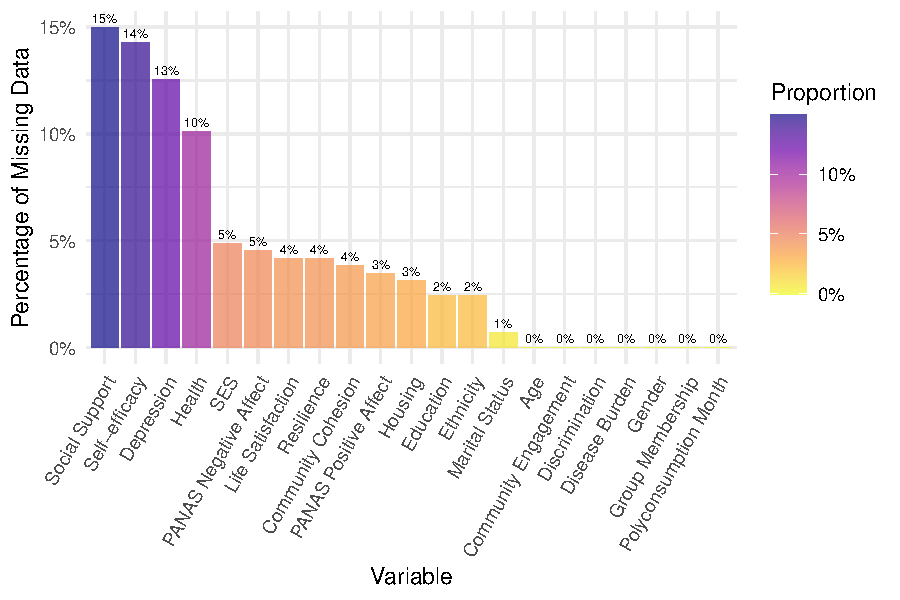
\includegraphics{Supplementary_material_files/figure-latex/fig-missing-data-1.pdf}
\caption{\label{fig:fig-missing-data}Proportion of missing data per variable. Variables are ordered from highest to lowest proportion of missing values. The color gradient indicates the proportion of missingness, with darker shades representing higher percentages.}
\end{figure}

\section{Multi-model inference}\label{multi-model-inference}

XXXX

\subsection{Life Satisfaction model}\label{life-satisfaction-model}

XXXX

\begin{Shaded}
\begin{Highlighting}[]
\NormalTok{dat\_LS }\OtherTok{\textless{}{-}}\NormalTok{ data }\SpecialCharTok{|\textgreater{}} 
  \FunctionTok{select}\NormalTok{(Life\_Satisfaction, Age, Gender, Ethnicity, Marital\_Status, Education, Housing, }
\NormalTok{         Self\_Efficacy, Community\_Cohesion, Depression, Social\_Support, Polyconsumption\_Month,}
\NormalTok{         Disease\_Burden, Discrimination, Group\_Membership, Community\_Engagement)}\SpecialCharTok{|\textgreater{}} 
  \FunctionTok{drop\_na}\NormalTok{()}

\NormalTok{global\_LS }\OtherTok{\textless{}{-}} \FunctionTok{lm}\NormalTok{(Life\_Satisfaction }\SpecialCharTok{\textasciitilde{}}\NormalTok{ Age }\SpecialCharTok{+}\NormalTok{ Gender }\SpecialCharTok{+}\NormalTok{ Ethnicity }\SpecialCharTok{+}\NormalTok{ Marital\_Status }\SpecialCharTok{+}\NormalTok{ Education }\SpecialCharTok{+}
\NormalTok{                  Housing }\SpecialCharTok{+}\NormalTok{ Self\_Efficacy }\SpecialCharTok{+}\NormalTok{ Community\_Cohesion }\SpecialCharTok{+}\NormalTok{ Depression }\SpecialCharTok{+} 
\NormalTok{                  Social\_Support }\SpecialCharTok{+}\NormalTok{ Polyconsumption\_Month }\SpecialCharTok{+}\NormalTok{ Disease\_Burden }\SpecialCharTok{+}\NormalTok{ Discrimination }\SpecialCharTok{+}
\NormalTok{                  Group\_Membership }\SpecialCharTok{+}\NormalTok{ Community\_Engagement,}
                \AttributeTok{data =}\NormalTok{ dat\_LS,}
                \AttributeTok{na.action =} \StringTok{"na.fail"}\NormalTok{)}
\end{Highlighting}
\end{Shaded}

\subsubsection{Dredge}\label{dredge}

XXXX

\begin{Shaded}
\begin{Highlighting}[]
\NormalTok{dr\_LS}\OtherTok{\textless{}{-}} \FunctionTok{dredge}\NormalTok{(global\_LS, }
               \AttributeTok{trace =} \DecValTok{2} \CommentTok{\#para ver barra de progreso}
\NormalTok{)}
\end{Highlighting}
\end{Shaded}

\begin{verbatim}
##   |                                                                              |                                                                      |   0%  |                                                                              |                                                                      |   1%  |                                                                              |=                                                                     |   1%  |                                                                              |=                                                                     |   2%  |                                                                              |==                                                                    |   2%  |                                                                              |==                                                                    |   3%  |                                                                              |==                                                                    |   4%  |                                                                              |===                                                                   |   4%  |                                                                              |===                                                                   |   5%  |                                                                              |====                                                                  |   5%  |                                                                              |====                                                                  |   6%  |                                                                              |=====                                                                 |   6%  |                                                                              |=====                                                                 |   7%  |                                                                              |=====                                                                 |   8%  |                                                                              |======                                                                |   8%  |                                                                              |======                                                                |   9%  |                                                                              |=======                                                               |   9%  |                                                                              |=======                                                               |  10%  |                                                                              |=======                                                               |  11%  |                                                                              |========                                                              |  11%  |                                                                              |========                                                              |  12%  |                                                                              |=========                                                             |  12%  |                                                                              |=========                                                             |  13%  |                                                                              |=========                                                             |  14%  |                                                                              |==========                                                            |  14%  |                                                                              |==========                                                            |  15%  |                                                                              |===========                                                           |  15%  |                                                                              |===========                                                           |  16%  |                                                                              |============                                                          |  16%  |                                                                              |============                                                          |  17%  |                                                                              |============                                                          |  18%  |                                                                              |=============                                                         |  18%  |                                                                              |=============                                                         |  19%  |                                                                              |==============                                                        |  19%  |                                                                              |==============                                                        |  20%  |                                                                              |==============                                                        |  21%  |                                                                              |===============                                                       |  21%  |                                                                              |===============                                                       |  22%  |                                                                              |================                                                      |  22%  |                                                                              |================                                                      |  23%  |                                                                              |================                                                      |  24%  |                                                                              |=================                                                     |  24%  |                                                                              |=================                                                     |  25%  |                                                                              |==================                                                    |  25%  |                                                                              |==================                                                    |  26%  |                                                                              |===================                                                   |  26%  |                                                                              |===================                                                   |  27%  |                                                                              |===================                                                   |  28%  |                                                                              |====================                                                  |  28%  |                                                                              |====================                                                  |  29%  |                                                                              |=====================                                                 |  29%  |                                                                              |=====================                                                 |  30%  |                                                                              |=====================                                                 |  31%  |                                                                              |======================                                                |  31%  |                                                                              |======================                                                |  32%  |                                                                              |=======================                                               |  32%  |                                                                              |=======================                                               |  33%  |                                                                              |=======================                                               |  34%  |                                                                              |========================                                              |  34%  |                                                                              |========================                                              |  35%  |                                                                              |=========================                                             |  35%  |                                                                              |=========================                                             |  36%  |                                                                              |==========================                                            |  36%  |                                                                              |==========================                                            |  37%  |                                                                              |==========================                                            |  38%  |                                                                              |===========================                                           |  38%  |                                                                              |===========================                                           |  39%  |                                                                              |============================                                          |  39%  |                                                                              |============================                                          |  40%  |                                                                              |============================                                          |  41%  |                                                                              |=============================                                         |  41%  |                                                                              |=============================                                         |  42%  |                                                                              |==============================                                        |  42%  |                                                                              |==============================                                        |  43%  |                                                                              |==============================                                        |  44%  |                                                                              |===============================                                       |  44%  |                                                                              |===============================                                       |  45%  |                                                                              |================================                                      |  45%  |                                                                              |================================                                      |  46%  |                                                                              |=================================                                     |  46%  |                                                                              |=================================                                     |  47%  |                                                                              |=================================                                     |  48%  |                                                                              |==================================                                    |  48%  |                                                                              |==================================                                    |  49%  |                                                                              |===================================                                   |  49%  |                                                                              |===================================                                   |  50%  |                                                                              |===================================                                   |  51%  |                                                                              |====================================                                  |  51%  |                                                                              |====================================                                  |  52%  |                                                                              |=====================================                                 |  52%  |                                                                              |=====================================                                 |  53%  |                                                                              |=====================================                                 |  54%  |                                                                              |======================================                                |  54%  |                                                                              |======================================                                |  55%  |                                                                              |=======================================                               |  55%  |                                                                              |=======================================                               |  56%  |                                                                              |========================================                              |  56%  |                                                                              |========================================                              |  57%  |                                                                              |========================================                              |  58%  |                                                                              |=========================================                             |  58%  |                                                                              |=========================================                             |  59%  |                                                                              |==========================================                            |  59%  |                                                                              |==========================================                            |  60%  |                                                                              |==========================================                            |  61%  |                                                                              |===========================================                           |  61%  |                                                                              |===========================================                           |  62%  |                                                                              |============================================                          |  62%  |                                                                              |============================================                          |  63%  |                                                                              |============================================                          |  64%  |                                                                              |=============================================                         |  64%  |                                                                              |=============================================                         |  65%  |                                                                              |==============================================                        |  65%  |                                                                              |==============================================                        |  66%  |                                                                              |===============================================                       |  66%  |                                                                              |===============================================                       |  67%  |                                                                              |===============================================                       |  68%  |                                                                              |================================================                      |  68%  |                                                                              |================================================                      |  69%  |                                                                              |=================================================                     |  69%  |                                                                              |=================================================                     |  70%  |                                                                              |=================================================                     |  71%  |                                                                              |==================================================                    |  71%  |                                                                              |==================================================                    |  72%  |                                                                              |===================================================                   |  72%  |                                                                              |===================================================                   |  73%  |                                                                              |===================================================                   |  74%  |                                                                              |====================================================                  |  74%  |                                                                              |====================================================                  |  75%  |                                                                              |=====================================================                 |  75%  |                                                                              |=====================================================                 |  76%  |                                                                              |======================================================                |  76%  |                                                                              |======================================================                |  77%  |                                                                              |======================================================                |  78%  |                                                                              |=======================================================               |  78%  |                                                                              |=======================================================               |  79%  |                                                                              |========================================================              |  79%  |                                                                              |========================================================              |  80%  |                                                                              |========================================================              |  81%  |                                                                              |=========================================================             |  81%  |                                                                              |=========================================================             |  82%  |                                                                              |==========================================================            |  82%  |                                                                              |==========================================================            |  83%  |                                                                              |==========================================================            |  84%  |                                                                              |===========================================================           |  84%  |                                                                              |===========================================================           |  85%  |                                                                              |============================================================          |  85%  |                                                                              |============================================================          |  86%  |                                                                              |=============================================================         |  86%  |                                                                              |=============================================================         |  87%  |                                                                              |=============================================================         |  88%  |                                                                              |==============================================================        |  88%  |                                                                              |==============================================================        |  89%  |                                                                              |===============================================================       |  89%  |                                                                              |===============================================================       |  90%  |                                                                              |===============================================================       |  91%  |                                                                              |================================================================      |  91%  |                                                                              |================================================================      |  92%  |                                                                              |=================================================================     |  92%  |                                                                              |=================================================================     |  93%  |                                                                              |=================================================================     |  94%  |                                                                              |==================================================================    |  94%  |                                                                              |==================================================================    |  95%  |                                                                              |===================================================================   |  95%  |                                                                              |===================================================================   |  96%  |                                                                              |====================================================================  |  96%  |                                                                              |====================================================================  |  97%  |                                                                              |====================================================================  |  98%  |                                                                              |===================================================================== |  98%  |                                                                              |===================================================================== |  99%  |                                                                              |======================================================================|  99%  |                                                                              |======================================================================| 100%
\end{verbatim}

\paragraph{Fig. \ref{fig:fig-dredge-LS}. Dredge results of the Life Satisfaction model}\label{fig.-reffigfig-dredge-ls.-dredge-results-of-the-life-satisfaction-model}

XXXX

\begin{Shaded}
\begin{Highlighting}[]
\FunctionTok{plot}\NormalTok{(dr\_LS[}\DecValTok{1}\SpecialCharTok{:}\DecValTok{100}\NormalTok{,])}
\end{Highlighting}
\end{Shaded}

\begin{figure}
\centering
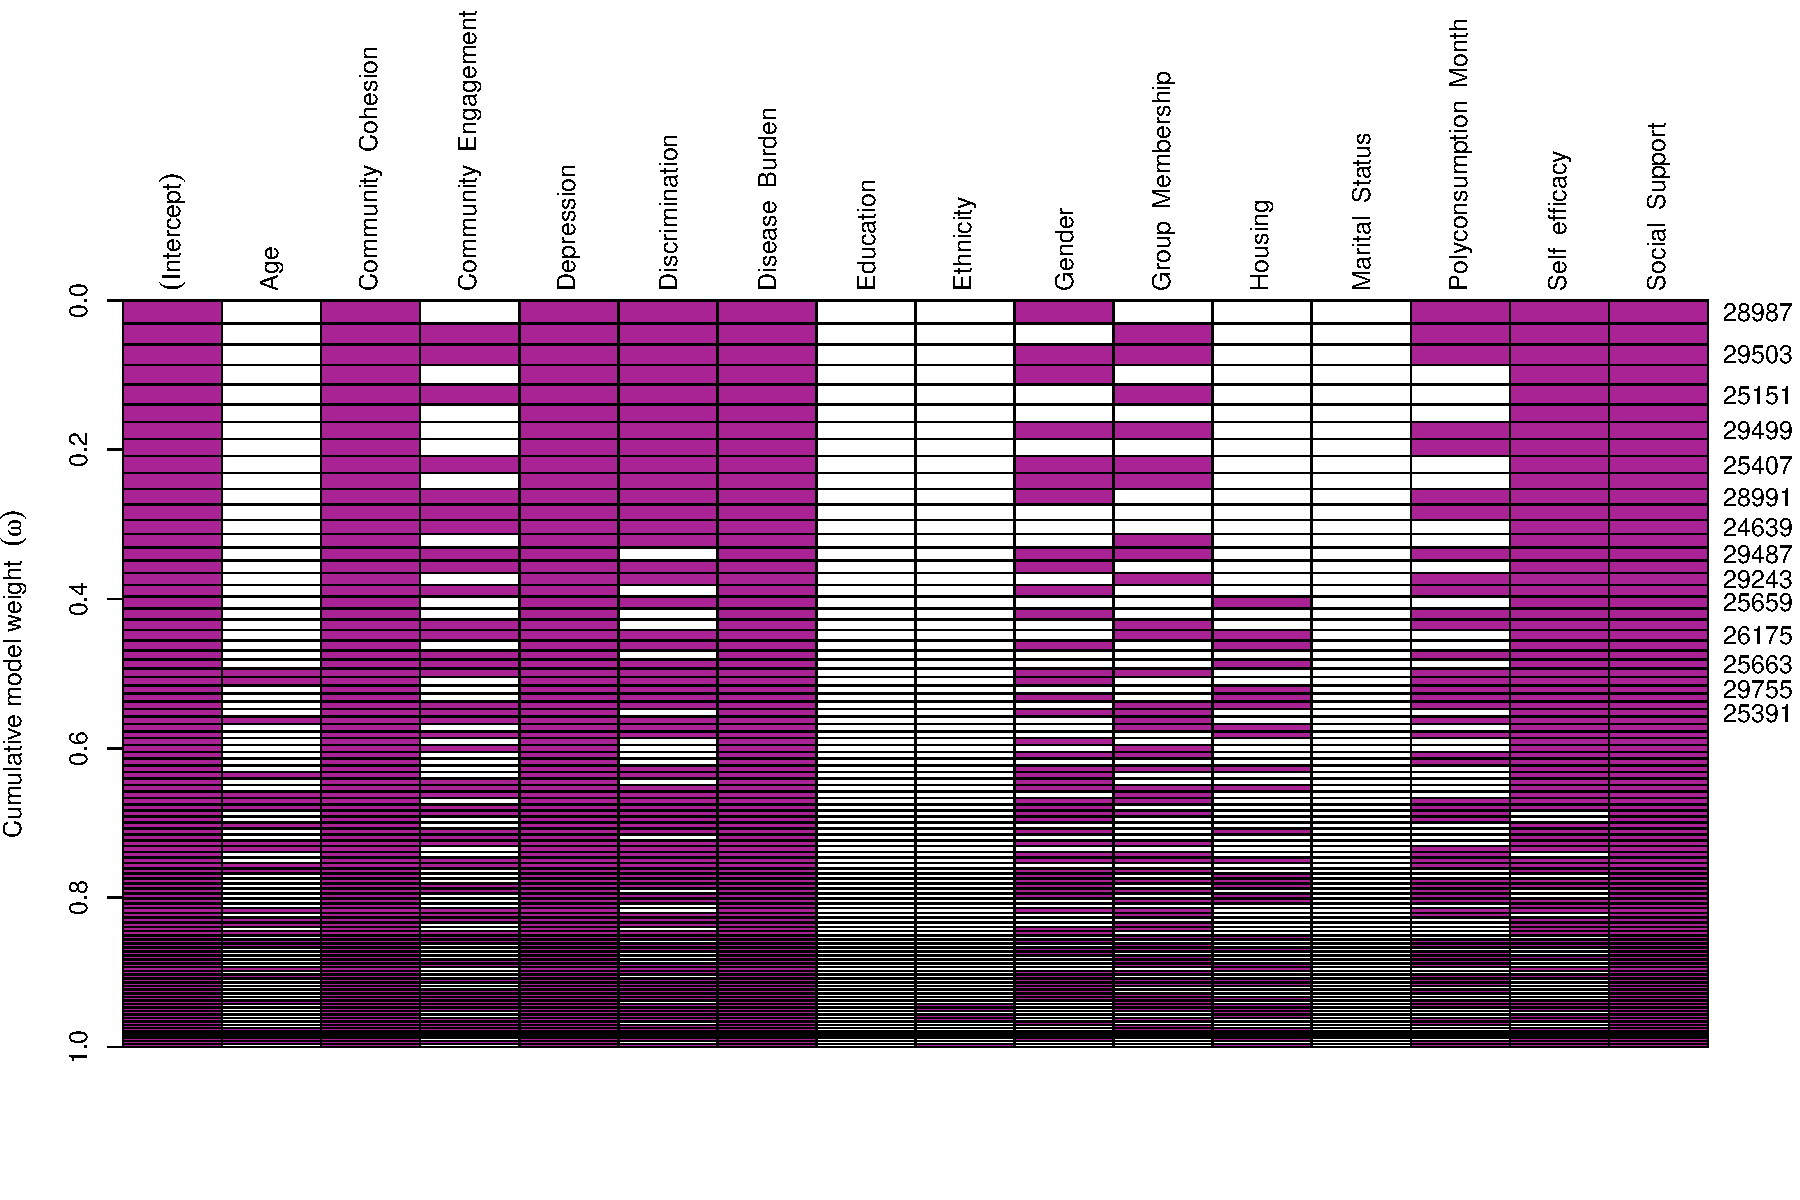
\includegraphics{Supplementary_material_files/figure-latex/fig-dredge-LS-1.pdf}
\caption{\label{fig:fig-dredge-LS}XXXX.}
\end{figure}

\subsubsection{Average model}\label{average-model}

XXXX

\begin{Shaded}
\begin{Highlighting}[]
\NormalTok{avg\_LS }\OtherTok{\textless{}{-}} \FunctionTok{model.avg}\NormalTok{(dr\_LS, }\AttributeTok{subset =}\NormalTok{ delta }\SpecialCharTok{\textless{}} \DecValTok{2}\NormalTok{, }\AttributeTok{fit =} \ConstantTok{TRUE}\NormalTok{)}
\end{Highlighting}
\end{Shaded}

\paragraph{Table \ref{tab:tab-avg-LS}. XXXX}\label{table-reftabtab-avg-ls.-xxxx}

XXXX

\begin{Shaded}
\begin{Highlighting}[]
\FunctionTok{avg.model.anova}\NormalTok{(avg\_LS, }\AttributeTok{data =}\NormalTok{ dat\_LS, }\AttributeTok{response =} \StringTok{"Life\_Satisfaction"}\NormalTok{)}
\end{Highlighting}
\end{Shaded}

\begin{table}[H]
\centering
\caption{\label{tab:tab-avg-LS}XXXXXX}
\centering
\begin{threeparttable}
\begin{tabular}[t]{lcccc}
\toprule
Term & $SS_{term}$ & $df$ & $F$ & $p$\\
\midrule
(Intercept) & 45.147 & 1, 193 & 23.014 & \textbf{< 0.0001}\\
Community Cohesion & 20.366 & 1, 193 & 10.382 & \textbf{0.0015}\\
Depression & 18.169 & 1, 193 & 9.262 & \textbf{0.0027}\\
Discrimination & 6.953 & 1, 193 & 3.544 & 0.06\\
Disease Burden & 13.223 & 1, 193 & 6.740 & \textbf{0.0102}\\
Polyconsumption Month & 4.738 & 1, 193 & 2.415 & 0.12\\
Self Efficacy & 10.125 & 1, 193 & 5.161 & \textbf{0.0242}\\
Social Support & 20.028 & 1, 193 & 10.209 & \textbf{0.0016}\\
Community Engagement & 6.513 & 1, 193 & 3.320 & 0.07\\
Group Membership & 5.470 & 1, 193 & 2.788 & 0.1\\
Age & 0.363 & 1, 193 & 0.185 & 0.67\\
\bottomrule
\end{tabular}
\begin{tablenotes}[para]
\item \textit{Note: } 
\item This ANOVA table was generated based on model-averaged estimates from 
      multimodel inference. The predictor terms included in the model were selected based on 
      their relative importance across candidate models ($\Delta AICc$ < 2). 
      Sum of squares ($SS_{term}$) values correspond to Type III ANOVA calculations, 
      which test each term's contribution while controlling for all other predictors. 
      Degrees of freedom ($df$) are presented as term $df$ and residual $df$, where residual 
      $df$ reflects the remaining degrees of freedom in the model. The $F$ and $p$ values were
      computed from the refitted model using only the selected predictors.
      Significant effects are in bold.
\end{tablenotes}
\end{threeparttable}
\end{table}

\paragraph{Fig. \ref{fig:fig-avg-LS}. Dredge results of the Life Satisfaction model}\label{fig.-reffigfig-avg-ls.-dredge-results-of-the-life-satisfaction-model}

XXXX

\begin{Shaded}
\begin{Highlighting}[]
\FunctionTok{avg.mod.plot}\NormalTok{(avg\_LS)}
\end{Highlighting}
\end{Shaded}

\begin{figure}
\centering
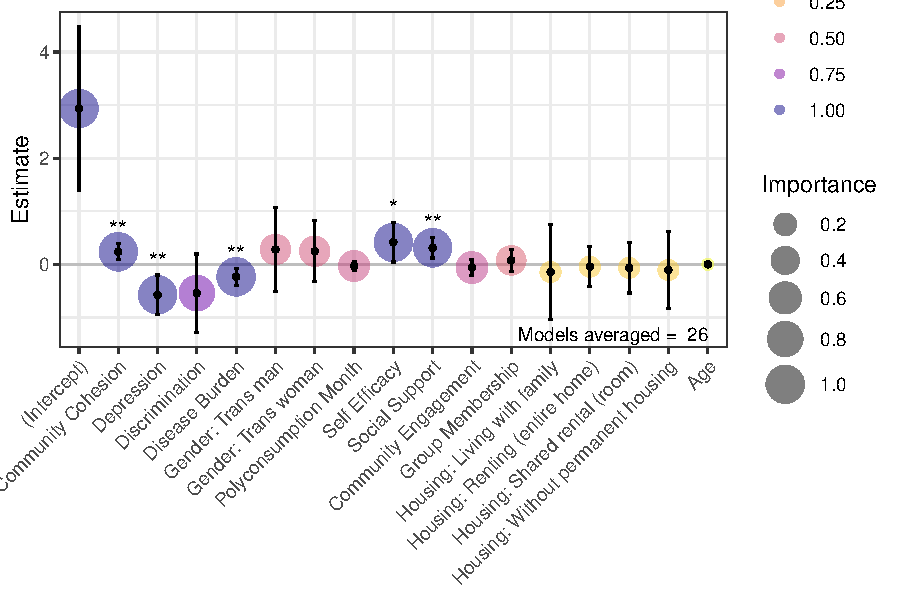
\includegraphics{Supplementary_material_files/figure-latex/fig-avg-LS-1.pdf}
\caption{\label{fig:fig-avg-LS}XXXX.}
\end{figure}

\begin{center}\rule{0.5\linewidth}{0.5pt}\end{center}

\section{Session info (for reproducibility)}\label{session}

\begin{Shaded}
\begin{Highlighting}[]
\CommentTok{\# Display session information for reproducibility}
\CommentTok{\# {-} Uses \textasciigrave{}pander()\textasciigrave{} for better formatting}
\CommentTok{\# {-} \textasciigrave{}locale = FALSE\textasciigrave{} to exclude locale{-}specific info (reduces clutter)}
\FunctionTok{library}\NormalTok{(pander)}
\FunctionTok{pander}\NormalTok{(}\FunctionTok{sessionInfo}\NormalTok{(), }\AttributeTok{locale =} \ConstantTok{FALSE}\NormalTok{)}
\end{Highlighting}
\end{Shaded}

\textbf{R version 4.4.3 (2025-02-28)}

\textbf{Platform:} x86\_64-pc-linux-gnu

\textbf{attached base packages:}
\emph{stats}, \emph{graphics}, \emph{grDevices}, \emph{utils}, \emph{datasets}, \emph{methods} and \emph{base}

\textbf{other attached packages:}
\emph{pander(v.0.6.6)}, \emph{lubridate(v.1.9.4)}, \emph{forcats(v.1.0.0)}, \emph{stringr(v.1.5.1)}, \emph{dplyr(v.1.1.4)}, \emph{purrr(v.1.0.4)}, \emph{tidyr(v.1.3.1)}, \emph{tibble(v.3.2.1)}, \emph{ggplot2(v.3.5.1)}, \emph{tidyverse(v.2.0.0)}, \emph{car(v.3.1-3)}, \emph{carData(v.3.0-5)}, \emph{kableExtra(v.1.4.0)}, \emph{scales(v.1.3.0)}, \emph{readr(v.2.1.5)}, \emph{performance(v.0.13.0)}, \emph{MuMIn(v.1.48.4)}, \emph{psych(v.2.4.12)}, \emph{ltm(v.1.2-0)}, \emph{polycor(v.0.8-1)}, \emph{msm(v.1.8.2)}, \emph{MASS(v.7.3-64)} and \emph{knitr(v.1.49)}

\textbf{loaded via a namespace (and not attached):}
\emph{gtable(v.0.3.6)}, \emph{xfun(v.0.51)}, \emph{insight(v.1.1.0)}, \emph{lattice(v.0.22-6)}, \emph{tzdb(v.0.4.0)}, \emph{vctrs(v.0.6.5)}, \emph{tools(v.4.4.3)}, \emph{generics(v.0.1.3)}, \emph{stats4(v.4.4.3)}, \emph{parallel(v.4.4.3)}, \emph{pkgconfig(v.2.0.3)}, \emph{Matrix(v.1.7-2)}, \emph{lifecycle(v.1.0.4)}, \emph{farver(v.2.1.2)}, \emph{compiler(v.4.4.3)}, \emph{munsell(v.0.5.1)}, \emph{mnormt(v.2.1.1)}, \emph{htmltools(v.0.5.8.1)}, \emph{yaml(v.2.3.10)}, \emph{Formula(v.1.2-5)}, \emph{crayon(v.1.5.3)}, \emph{pillar(v.1.10.1)}, \emph{admisc(v.0.37)}, \emph{abind(v.1.4-8)}, \emph{nlme(v.3.1-167)}, \emph{tidyselect(v.1.2.1)}, \emph{digest(v.0.6.37)}, \emph{mvtnorm(v.1.3-3)}, \emph{stringi(v.1.8.4)}, \emph{bookdown(v.0.42)}, \emph{labeling(v.0.4.3)}, \emph{splines(v.4.4.3)}, \emph{fastmap(v.1.2.0)}, \emph{grid(v.4.4.3)}, \emph{archive(v.1.1.11)}, \emph{colorspace(v.2.1-1)}, \emph{expm(v.1.0-0)}, \emph{cli(v.3.6.3)}, \emph{magrittr(v.2.0.3)}, \emph{survival(v.3.8-3)}, \emph{broom(v.1.0.7)}, \emph{withr(v.3.0.2)}, \emph{backports(v.1.5.0)}, \emph{bit64(v.4.6.0-1)}, \emph{timechange(v.0.3.0)}, \emph{rmarkdown(v.2.29)}, \emph{bit(v.4.5.0.1)}, \emph{hms(v.1.1.3)}, \emph{evaluate(v.1.0.3)}, \emph{viridisLite(v.0.4.2)}, \emph{rlang(v.1.1.5)}, \emph{Rcpp(v.1.0.14)}, \emph{glue(v.1.8.0)}, \emph{xml2(v.1.3.6)}, \emph{vroom(v.1.6.5)}, \emph{svglite(v.2.1.3)}, \emph{rstudioapi(v.0.17.1)}, \emph{R6(v.2.5.1)} and \emph{systemfonts(v.1.2.1)}

\begin{center}\rule{0.5\linewidth}{0.5pt}\end{center}

\section{Supplementary references}\label{refs}

\begin{multicols}{2}
\AtNextBibliography{\footnotesize}
\printbibliography[heading=none]
\normalsize
\end{multicols}

\def\printbibliography{}

\printbibliography

\end{document}
